\documentclass{ieeeaccess}
\usepackage{cite}
\usepackage{amsmath,amssymb,amsfonts}
\usepackage{algorithmic}
\usepackage{graphicx}
\usepackage{textcomp}
\usepackage{booktabs}
\usepackage{multirow}
\usepackage{array}

\def\BibTeX{{\rm B\kern-.05em{\sc i\kern-.025em b}\kern-.08em
    T\kern-.1667em\lower.7ex\hbox{E}\kern-.125emX}}

\begin{document}
\history{This manuscript draft is prepared for internal review before submission.}
\doi{}

\title{An End-to-End Multimodal AI Framework for Power Data Asset Valuation and Trading}
\author{\uppercase{Xingchen Li}\authorrefmark{1}, and \uppercase{Jijun Wang}\authorrefmark{2}}
\address[1]{Affiliation to be added before submission (e-mail: to be added)}
\address[2]{Affiliation to be added before submission (e-mail: to be added)}
\tfootnote{This work received no external funding.}

\markboth
{Author \headeretal: End-to-End Multimodal AI Framework for Power Data Asset Valuation and Trading}
{Author \headeretal: End-to-End Multimodal AI Framework for Power Data Asset Valuation and Trading}

\corresp{Corresponding author: Xingchen Li (e-mail: to be added).}

\begin{abstract}
As data has emerged as a vital production factor in modern power systems, the valuation and efficient trading of power data assets face significant challenges due to inherent heterogeneity, temporal dependency, market uncertainty, and privacy constraints. This paper proposes an end-to-end multimodal AI framework for power data asset markets rather than a standalone forecasting model. The framework integrates three functional modules: a multimodal proxy valuation module, a natural-language-assisted Deep Reinforcement Learning (DRL) matching module, and a differential-privacy utility stress-test module. First, TransModal-ValueNet uses cross-attention to fuse load profiles, market prices, weather features, renewable generation patterns, and temporal characteristics into multidimensional proxy value scores. Second, a query parser translates buyer requests into structured trading parameters, and a Soft Actor-Critic (SAC) policy optimizes peer-to-peer matching decisions. Third, a floor-smoothed heterogeneous differential privacy mechanism is evaluated against uniform budget allocation to quantify utility loss under private data release. The framework is validated using 8,777 hourly samples derived from full-year 2024 CAISO market data and Open-Meteo meteorological variables, together with a 20-microgrid P2P trading environment. The valuation experiment shows that XGBoost obtains the lowest single-target MAE (0.0297), Linear Regression obtains the highest R\textsuperscript{2} (0.118), and TransModal-ValueNet remains competitive in MAE (0.0313) but does not dominate all baselines under full-year LMP volatility. The packaged SAC trading agent attains 3.41$\times$ higher cumulative rewards than random matching with a 90.13\% deal rate, and three-seed retraining preserves a 3.21$\times$ mean reward advantage. The privacy experiment shows that uniform DP preserves 25.9\% value at $\varepsilon = 10$, exceeding the current smoothed adaptive allocation (16.9\%), revealing a practical boundary of static feature-importance-based privacy allocation. These results position the proposed system as a reproducible applied benchmark for power data asset trading, while further validation with real transaction prices and additional markets remains necessary.
\end{abstract}

\begin{keywords}
Data valuation, multimodal AI, power data trading, peer-to-peer matching, deep reinforcement learning, differential privacy, cross-attention Transformer, CAISO market.
\end{keywords}

\titlepgskip=-15pt

\maketitle

\section{Introduction}
\label{sec:introduction}
\PARstart{P}{ower} systems worldwide are undergoing a profound digital transformation, with smart meters, phasor measurement units, and advanced metering infrastructure generating unprecedented volumes of operational data. The State Council of China formally designated data as the fifth production factor in 2020 (alongside land, labor, capital, and technology), recognizing its strategic value for economic development \cite{b1}. Within the energy sector, power data---including load profiles, locational marginal prices (LMP), renewable generation outputs, and meteorological measurements---constitutes a high-value asset class whose proper valuation and trading could unlock significant economic efficiency.

However, several fundamental barriers impede the development of power data markets. First, \textit{data valuation} remains largely heuristic: existing approaches often rely on cost-based formulas or manually determined correction coefficients \cite{b2}, lacking the ability to capture dynamic, context-dependent value that varies with market conditions, time of day, and data quality. Second, \textit{trading efficiency} is constrained by manual matchmaking between data buyers and sellers, resulting in high transaction costs and low liquidity. Third, \textit{privacy concerns} create tension between data monetization and protection: noise injection through differential privacy degrades data utility, and practical market platforms need empirical tools to quantify this degradation. Fourth, \textit{multi-source heterogeneity}---load profiles, market prices, renewable generation, weather measurements, and temporal context---remains underutilized in data-asset trading workflows.

Recent advances in multimodal artificial intelligence offer promising avenues to address these challenges. Cross-attention Transformer architectures have demonstrated strong capability in fusing heterogeneous data modalities \cite{b3}. Pre-trained language models can support natural-language understanding and structured parameter extraction \cite{b4}. Deep Reinforcement Learning (DRL), particularly Soft Actor-Critic (SAC), has achieved strong performance in continuous control and market optimization problems \cite{b5}. Despite these advances, the integration of multimodal valuation, query understanding, trading optimization, and privacy-aware release remains underexplored for power data asset markets.

This paper proposes a comprehensive multimodal AI-driven framework that bridges this gap. The emphasis is not on claiming a universally superior forecasting architecture, but on building and stress-testing an integrated power-data-market workflow. Our key contributions are:

\begin{enumerate}
  \item \textbf{End-to-End Power Data Market Framework}: We integrate multimodal data valuation, natural-language demand parsing, DRL-based P2P matching, and privacy-utility evaluation into one reproducible workflow for power data asset trading.

  \item \textbf{Multimodal Valuation Benchmark}: We design TransModal-ValueNet, a cross-attention Transformer that fuses five power-system modalities---temporal features, load profiles, market prices, renewable generation patterns, and weather variables---to produce multidimensional proxy value scores. The benchmark includes strong tabular baselines and reports both positive and negative model findings under full-year LMP volatility.

  \item \textbf{Natural-Language-Assisted DRL Matching Engine}: A two-stage architecture where a Sentence-BERT/TF-IDF few-shot parser maps natural language queries into structured matching parameters, and a SAC agent optimizes sequential matching decisions in a continuous action space, achieving 3.41$\times$ improvement over random baselines in deterministic saved-model evaluation.

  \item \textbf{Heterogeneous Differential Privacy Stress Test}: A feature-importance-driven privacy budget allocation mechanism assigns differential epsilon budgets to each modality with a uniform floor. Under the full-year LMP setting, the experiment reveals that uniform DP remains stronger than the current adaptive allocation, providing a diagnostic boundary for future validation-aware privacy-utility optimization.

  \item \textbf{Full-Year Empirical Package}: We construct a multimodal dataset spanning 8,777 hourly samples derived from California ISO (CAISO) load, renewable generation, and full-year 2024 day-ahead LMP records at NP15, SP15, and ZP26 together with Open-Meteo meteorological data and a 20-microgrid P2P trading environment. After local-time alignment, one daylight-saving local hour is filled during fusion and all final modeled features contain no missing values.
\end{enumerate}

The remainder of this paper is organized as follows. Section II reviews related work in power data pricing, blockchain-enabled trading, multimodal AI in energy systems, and privacy-preserving data markets. Section III presents the system model and problem formulation. Section IV details the proposed framework, including TransModal-ValueNet, the natural-language-assisted DRL matching engine, and the privacy-utility co-optimizer. Section V describes the experimental setup, datasets, and baseline methods. Section VI reports and discusses experimental results. Section VII concludes the paper and outlines future research directions.

\section{Related Work}
\label{sec:related}

\subsection{Power Data Asset Pricing}
The pricing of data assets has been studied from several complementary perspectives, including query-based data markets, privacy-aware data pricing, and contribution-based data valuation. Query-based pricing formalizes how database answers can be priced while avoiding arbitrage \cite{b2,b6}. For machine-learning settings, data Shapley and its variants quantify each training sample's marginal contribution to model utility \cite{b7,b8}, while reinforcement-learning-based data valuation learns pricing policies from downstream performance feedback \cite{b9}. These studies provide useful foundations for valuing power data, but they are not tailored to power-system modalities such as load forecasts, locational marginal prices, renewable generation, and meteorological measurements.

\textbf{Limitation:} Existing data-valuation approaches provide important theoretical foundations, but they are rarely evaluated as part of an end-to-end power data trading workflow that includes multimodal feature construction, matching, and privacy-aware release.

\subsection{Blockchain-Enabled Power Data Trading}
Peer-to-peer electricity trading and blockchain-enabled energy markets have received extensive attention as mechanisms for decentralized coordination among distributed energy resources. Tushar \textit{et al.} \cite{b10} surveyed peer-to-peer trading architectures, pricing mechanisms, and network constraints in electricity networks. Mengelkamp \textit{et al.} \cite{b11} analyzed the Brooklyn Microgrid as a practical microgrid-market design case, while Kang \textit{et al.} \cite{b12} developed a consortium-blockchain mechanism for localized electricity trading among plug-in hybrid electric vehicles. Andoni \textit{et al.} \cite{b13} further reviewed blockchain opportunities and challenges across energy-sector applications.

\textbf{Limitation:} Existing blockchain and P2P energy trading studies mainly focus on physical electricity transactions. Their integration with data-asset valuation, query understanding, and privacy-aware data release remains limited.

\subsection{Multimodal AI in Energy Systems}
Recent forecasting literature increasingly combines heterogeneous time-series inputs through attention-based and foundation-model architectures. Temporal Fusion Transformers provide an interpretable attention architecture for multi-horizon forecasting with static and time-varying covariates \cite{b14}. Foundation time-series models such as Lag-Llama show the potential of pre-trained probabilistic forecasting models \cite{b15}. In electricity markets, comprehensive benchmarking has shown that forecasting accuracy depends strongly on data preprocessing, market-specific features, and model-selection protocols \cite{b16}. Multi-agent deep reinforcement learning methods such as MADDPG provide a general framework for strategic multi-agent decision-making \cite{b17}, while PatchTST demonstrates the effectiveness of Transformer-style patching for long-horizon time-series forecasting \cite{b18}.

\textbf{Limitation:} Compared with physical electricity trading, power \textit{data trading} remains underexplored. The use of multimodal information for data quality assessment, data asset valuation, and supply-demand matching is still at an early stage.

\subsection{Privacy-Preserving Data Markets}
Differential privacy (DP) has become a standard approach for privacy-preserving data release and machine learning \cite{b21,b22}. In smart-grid settings, \'{A}cs and Castelluccia \cite{b19} studied differentially private smart metering, and Fioretto \textit{et al.} \cite{b20} investigated DP-based obfuscation for power-grid data. These studies motivate privacy-preserving power data markets, but they generally apply privacy mechanisms uniformly rather than allocating privacy budgets according to modality-specific predictive utility.

\textbf{Limitation:} Existing privacy protection schemes for smart-grid data provide strong protection principles, but few studies report modality-aware privacy-budget stress tests for power data asset release under market-price volatility.

\section{System Model and Problem Formulation}
\label{sec:system}

\subsection{System Architecture}
The proposed framework operates within a power data marketplace comprising three stakeholder roles: \textit{data sellers} (utilities, grid operators, weather services) who offer datasets with metadata describing content, quality, and temporal coverage; \textit{data buyers} (researchers, traders, forecasting teams) who submit natural language queries specifying data requirements; and a \textit{market platform} that performs automated valuation, matching, and settlement. The system architecture consists of four layers:

\begin{enumerate}
  \item \textbf{Data Layer}: Multimodal data lake storing time-series power market data, renewable generation, weather measurements, temporal features, and P2P microgrid profiles.
  \item \textbf{AI Engine Layer}: Core intelligence layer containing TransModal-ValueNet for proxy valuation, the natural-language-assisted DRL engine for query understanding and matching, and the differential-privacy utility stress-test module.
  \item \textbf{Transaction Layer}: Smart-contract-based settlement and data asset registry with on-chain data fingerprints (hash + metadata summaries).
  \item \textbf{Application Layer}: User interfaces for data valuation dashboards, trading consoles, and quality audit panels.
\end{enumerate}

\begin{figure}[t!]
  \centering
  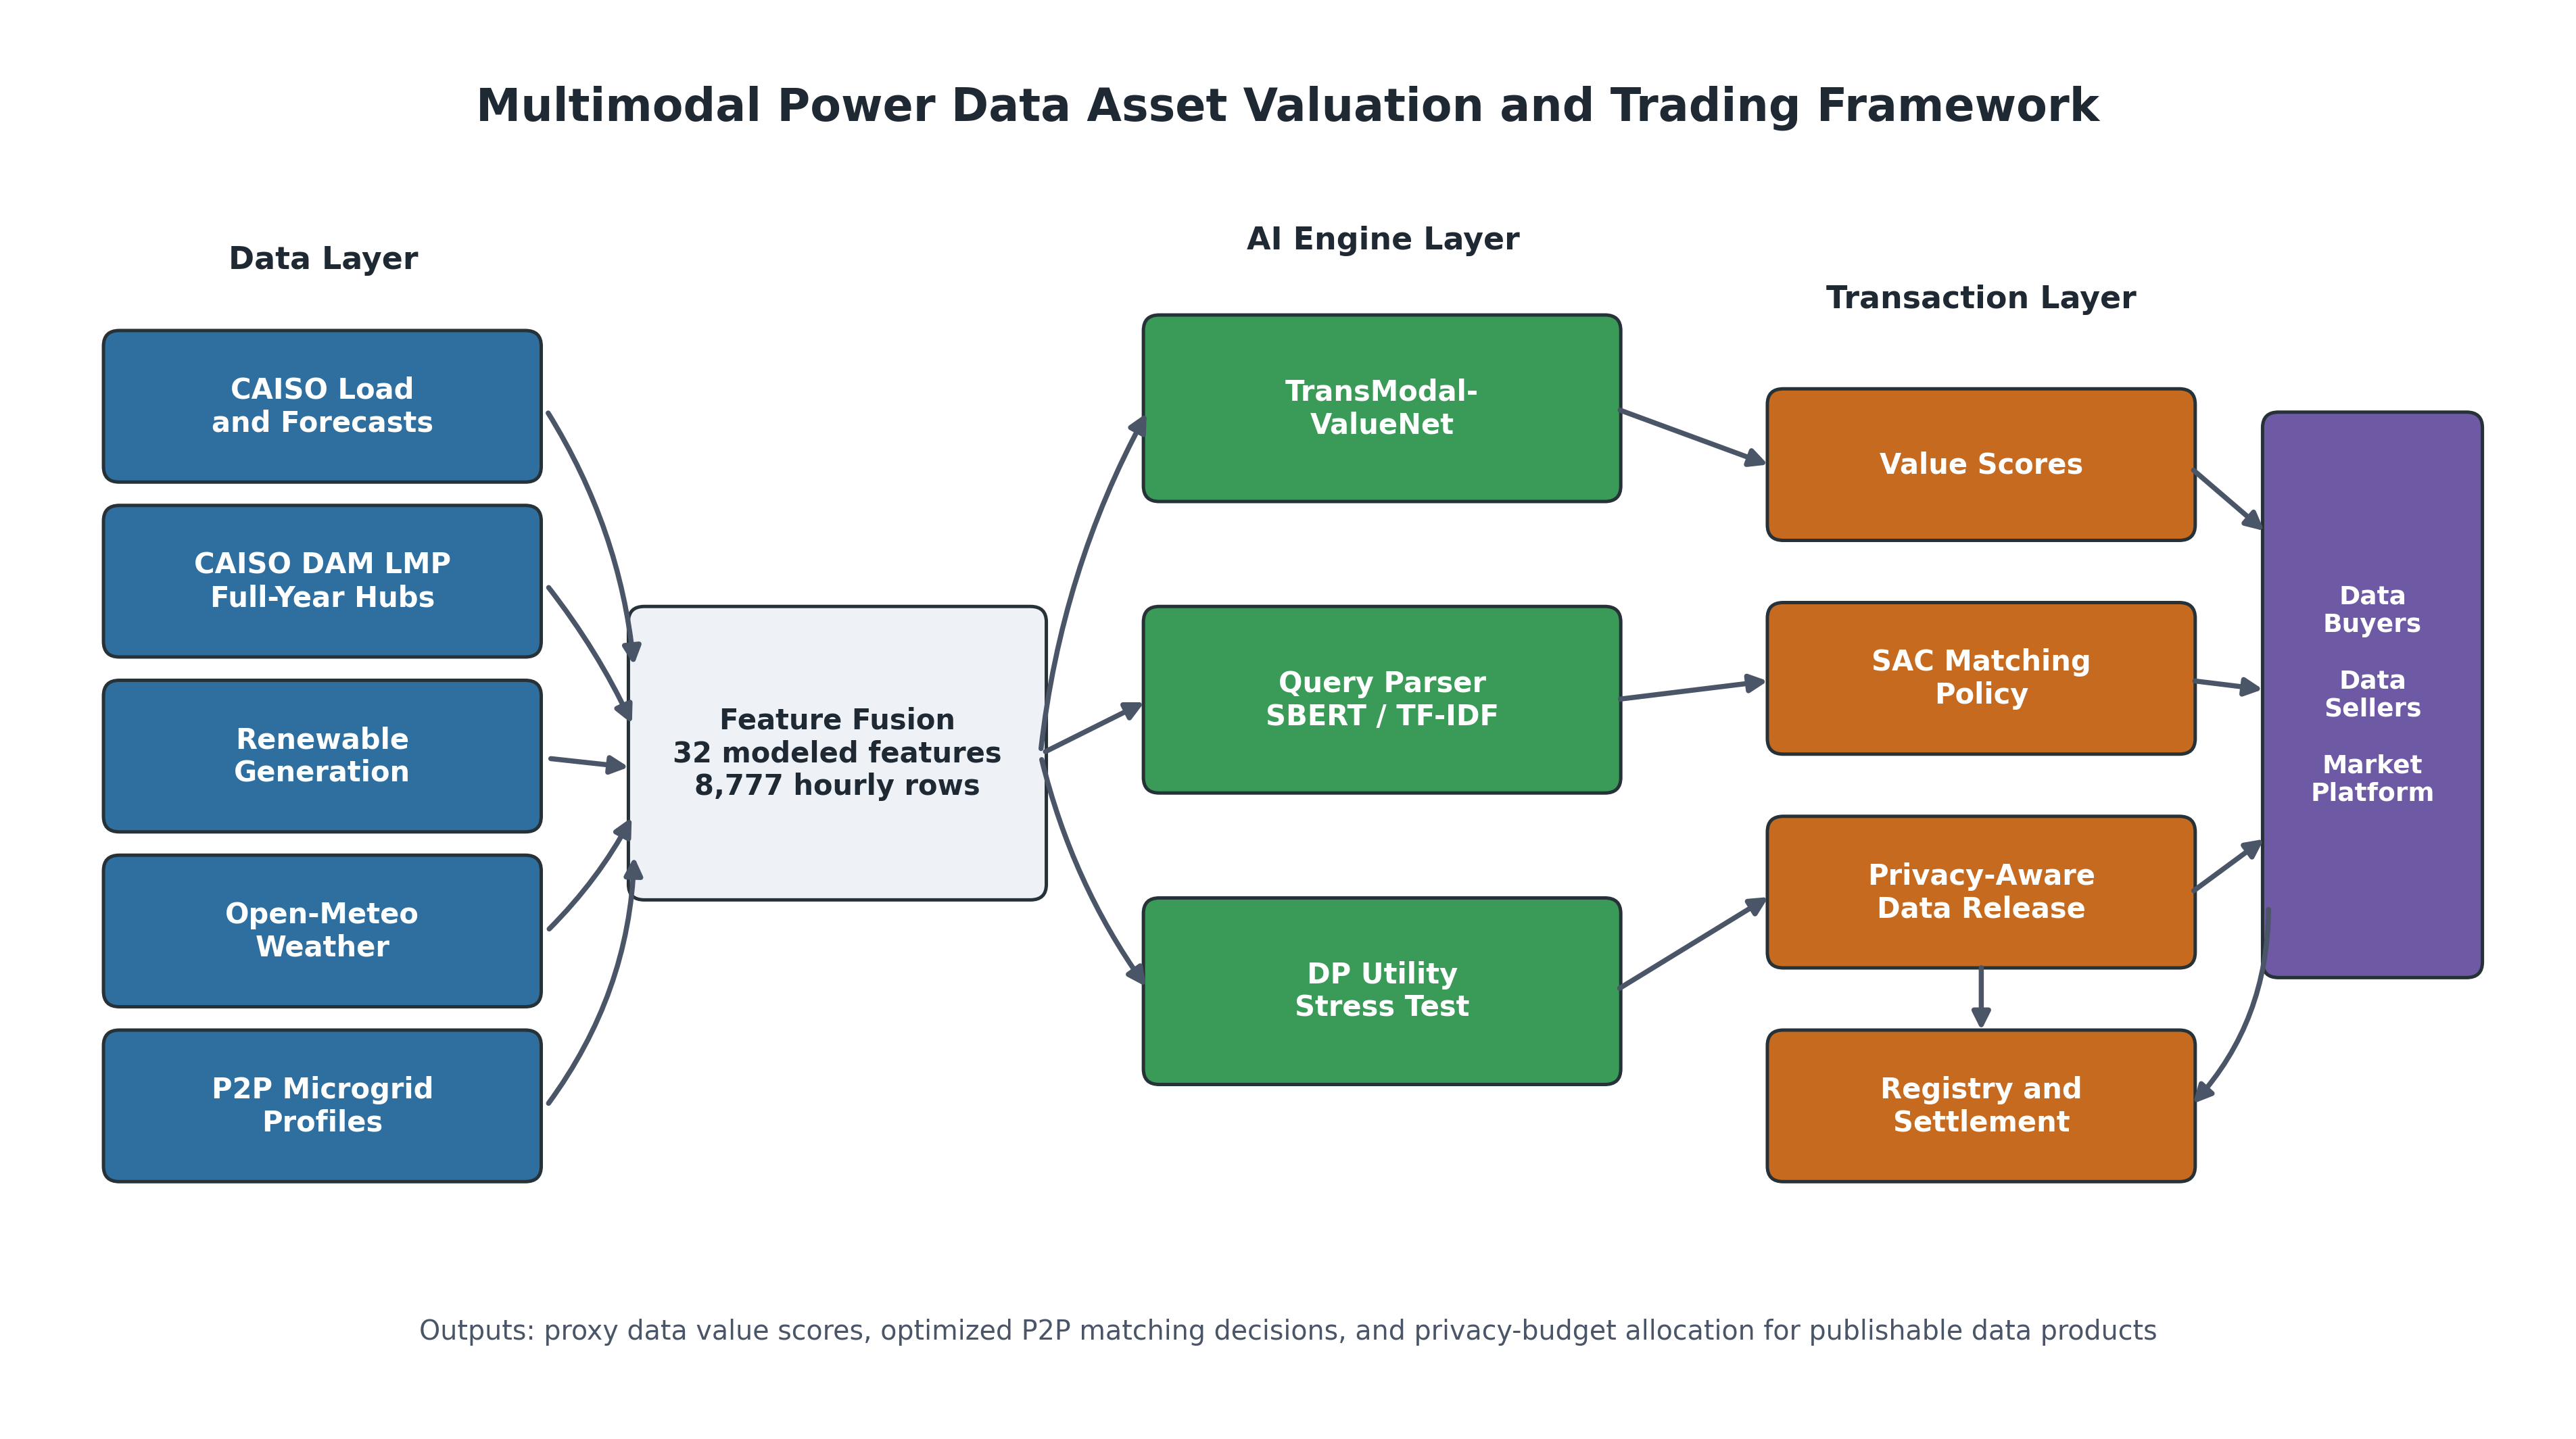
\includegraphics[width=0.98\columnwidth]{figures/system_architecture.png}
  \caption{System architecture of the proposed multimodal power data asset valuation and trading framework. The data layer feeds fused multimodal features to three AI modules: TransModal-ValueNet for proxy value scoring, a natural-language-assisted SAC matching engine, and a differential-privacy utility stress-test module.}
  \label{fig:system_arch}
\end{figure}

\subsection{Problem Formulation}
We formalize three core sub-problems addressed in this paper:

\textbf{Problem 1 (Multimodal Data Valuation):} Given a multivariate time series $\mathbf{X} = \{\mathbf{x}_t\}_{t=1}^T$ where each observation $\mathbf{x}_t = [\mathbf{x}_t^{(1)}, \ldots, \mathbf{x}_t^{(M)}]$ spans $M$ modalities (load, market, weather, generation, temporal), learn a valuation function $f_{\theta}: \mathbb{R}^{d_1} \times \cdots \times \mathbb{R}^{d_M} \rightarrow \mathbb{R}^4$ that maps modality observations to a 4-dimensional value score vector $v_t$. The four dimensions capture: (v1) day-ahead forecast error sensitivity, (v2) hour-ahead forecast error sensitivity, (v3) price volatility contribution, and (v4) renewable generation uncertainty premium.

\textbf{Problem 2 (Matching Optimization):} Given a set of buyers $B = \{b_1, \ldots, b_n\}$ with demand queries and sellers $S = \{s_1, \ldots, s_m\}$ with data offerings, learn a policy $\pi_{\phi}: \mathcal{S} \rightarrow \mathcal{A}$ that maps market state $s_t$ (net loads, hour, day, last clearing price) to matching actions $a_t$ (trading intensities per agent) to maximize cumulative social welfare $R = \sum_{t} r_t$, where $r_t$ represents the economic surplus from P2P trades relative to grid-only baselines.

\textbf{Problem 3 (Privacy-Utility Stress Testing):} Given a total privacy budget $\varepsilon_{total}$, compare uniform and heterogeneous allocations $\{\varepsilon_g\}_{g=1}^G$ across $G$ feature groups by measuring utility loss $\mathcal{L}(\varepsilon) = |R^2_{base} - R^2_{dp}(\varepsilon)|$, where $R^2_{dp}$ is the model performance under DP perturbation and $\sum_g \varepsilon_g \leq \varepsilon_{total}$ under $(\varepsilon, \delta)$-differential privacy.

\section{Proposed Framework}
\label{sec:framework}

\subsection{TransModal-ValueNet}
\label{sec:transmodal}

TransModal-ValueNet is a cross-attention Transformer architecture designed specifically for multimodal power data valuation. The key design challenge is that each modality has different dimensionality, statistical properties, and predictive relevance---requiring a flexible fusion mechanism.

\subsubsection{Architecture Design}

As illustrated in Fig.~\ref{fig:transmodal_arch}, the model comprises four components:

\begin{enumerate}
  \item \textbf{Modality Projection Layers}: Each modality $m$ with feature dimension $d_m$ is projected to a common hidden dimension $d_{\text{model}}=128$ via a linear layer $\mathbf{h}_m = \mathbf{W}_m \mathbf{x}_m + \mathbf{b}_m$. The five modalities are: temporal (4 features: hour, day of week, month, weekend indicator), load (3 features: demand, day-ahead forecast, hour-ahead forecast), market (4 features: LMP, energy, congestion, loss DAM prices), generation (6 features: solar, wind, geothermal, biomass, biogas, small hydro), and weather (15 features: temperature, humidity, dew point, apparent temperature, precipitation, pressure, cloud cover, radiation, wind speed/direction, soil moisture/temperature).

  \item \textbf{[CLS] Token and Cross-Attention Layers}: A learnable [CLS] token is prepended to the sequence of 5 modality tokens. The resulting 6-token sequence passes through $L=2$ transformer layers, each consisting of multi-head self-attention (4 heads, $d_{\text{model}}=128$), layer normalization, and a position-wise feed-forward network with GELU activation. The self-attention mechanism enables every modality to attend to every other modality, creating a fully expressive cross-modal representation.

  \item \textbf{Value Head}: After mean pooling across all 6 tokens, a 2-layer MLP ($128 \rightarrow 128 \rightarrow 4$) with GELU activation produces the 4-dimensional value score vector.

  \item \textbf{Reconstruction Heads (Pre-training Only)}: Per-modality linear layers project from $d_{\text{model}}$ back to $d_m$ for the masked autoencoder objective.
\end{enumerate}

\begin{figure}[t!]
  \centering
  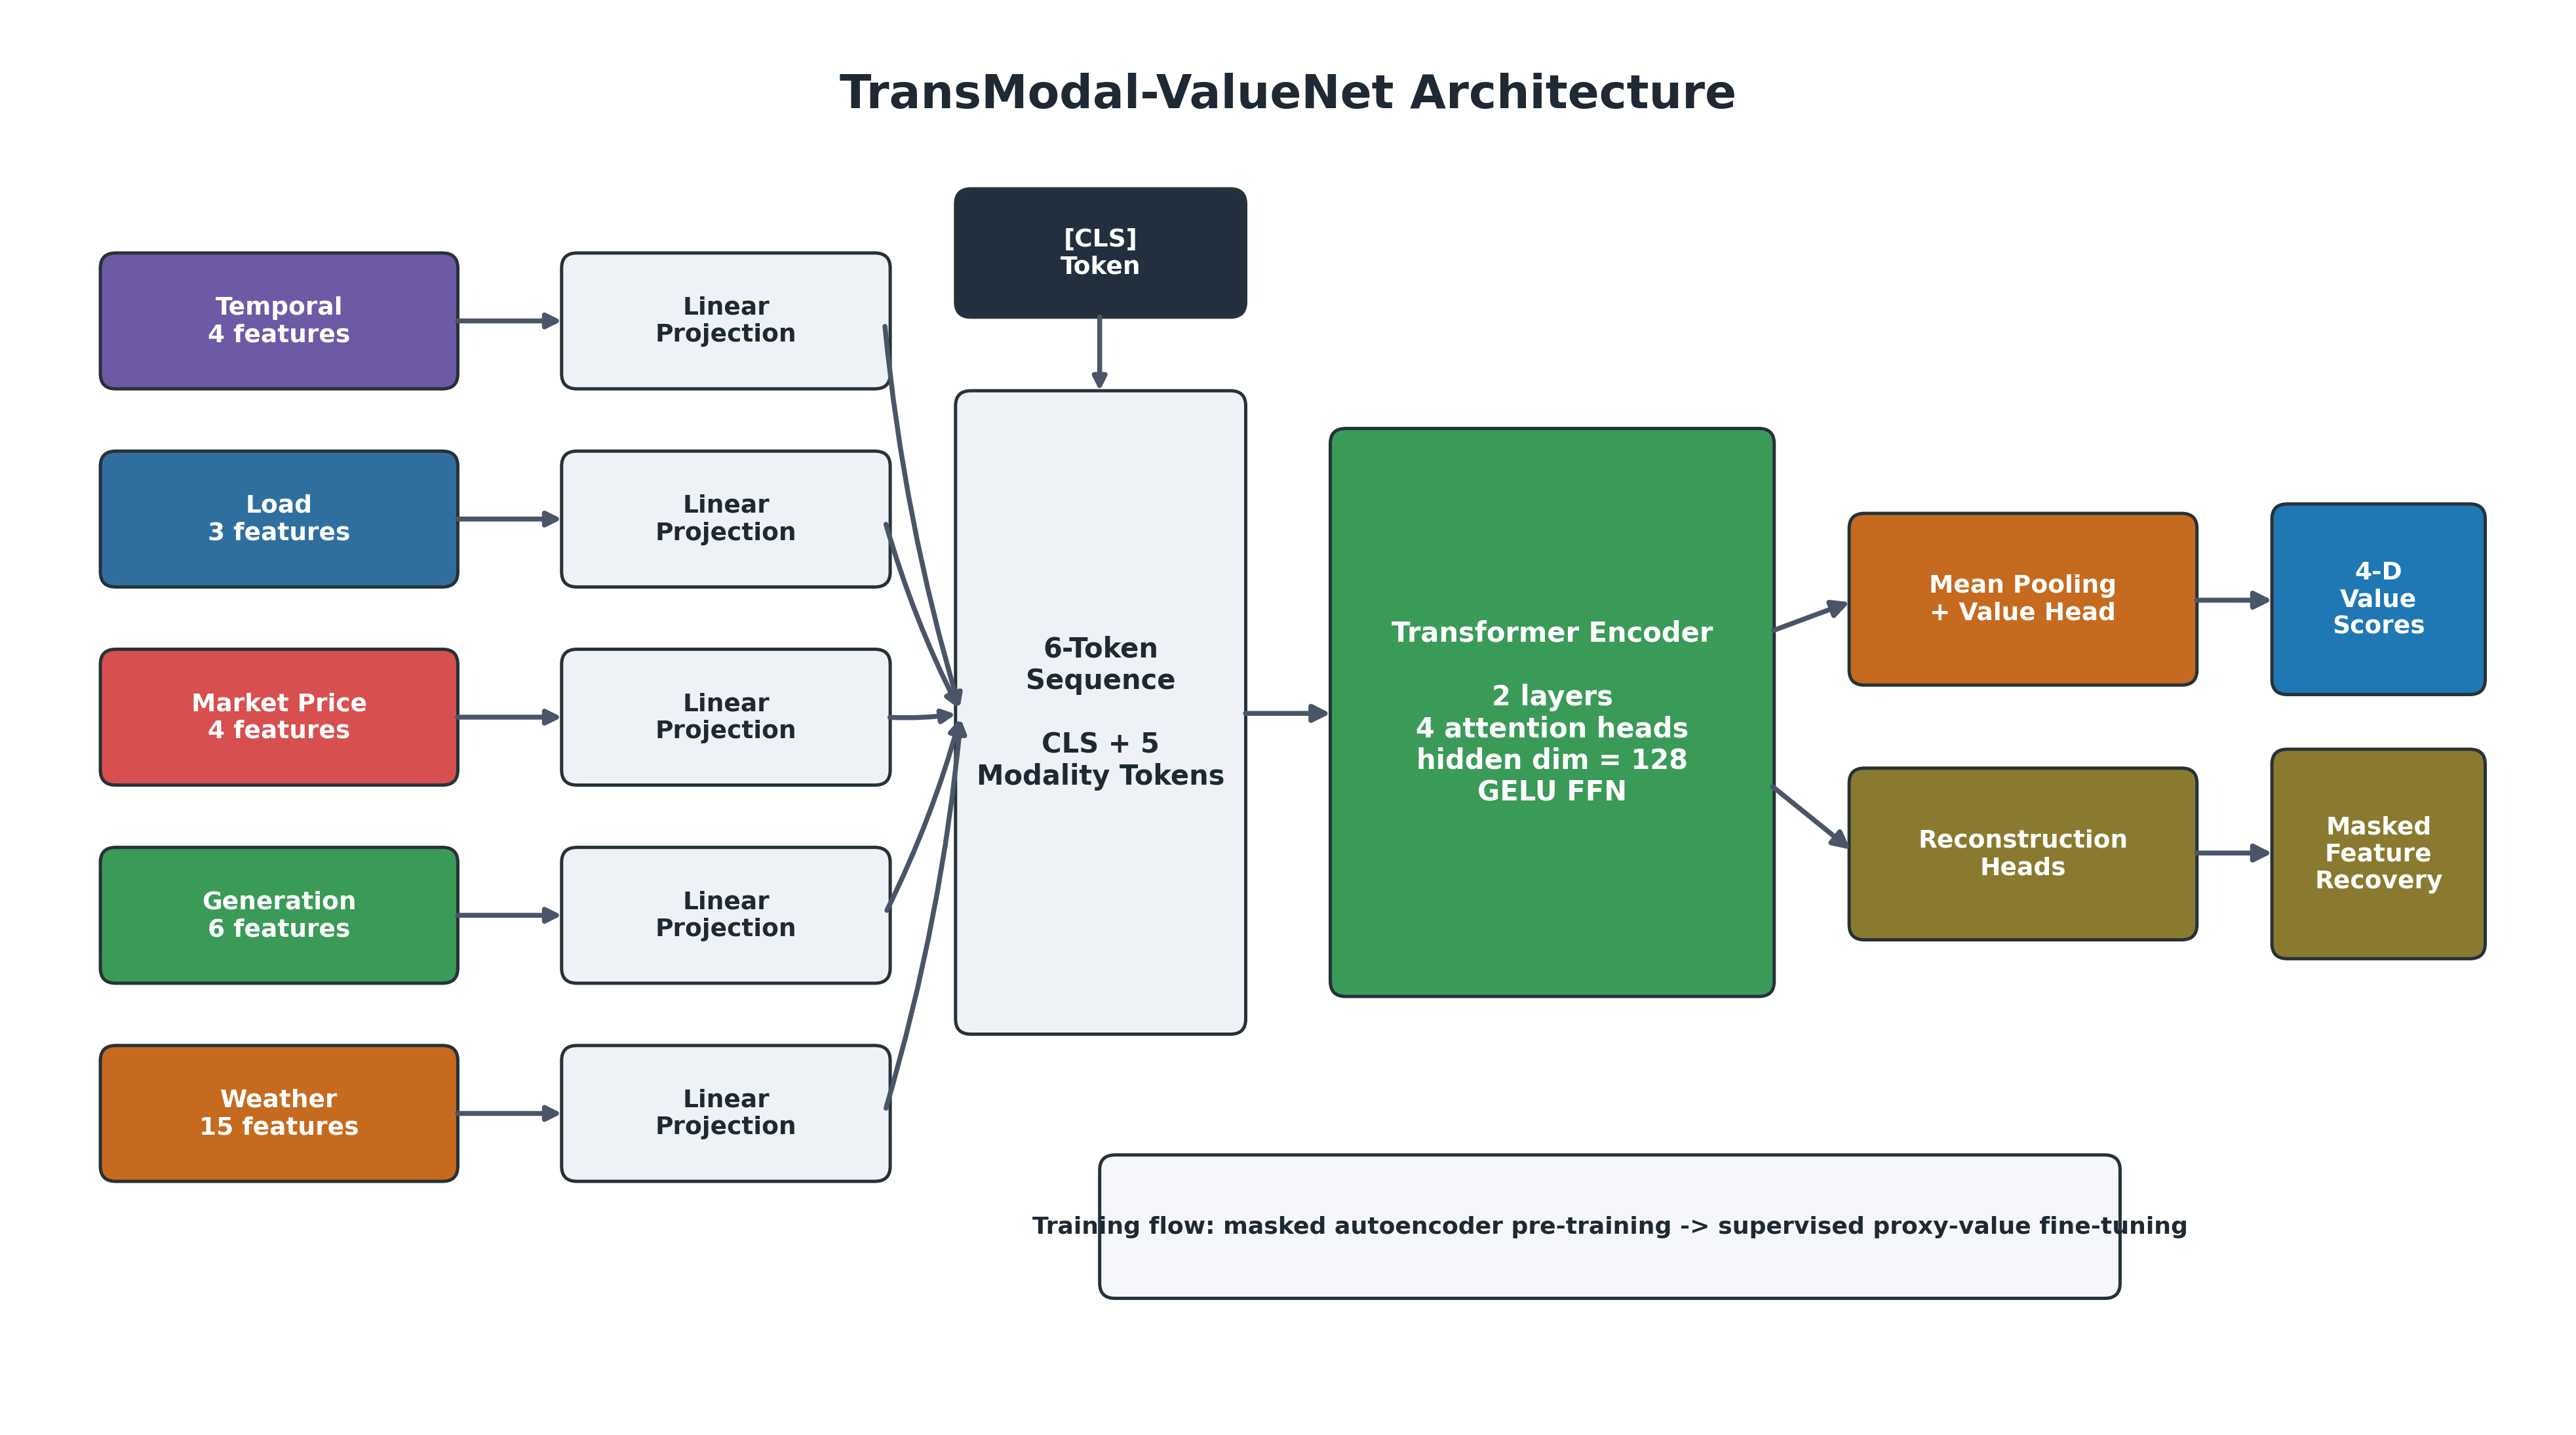
\includegraphics[width=0.98\columnwidth]{figures/transmodal_architecture.png}
  \caption{Architecture of TransModal-ValueNet. Five modality groups are projected to a common hidden dimension, concatenated with a learnable [CLS] token, processed by a Transformer encoder, and mapped to four proxy value-score dimensions. Reconstruction heads are used during masked-autoencoder pre-training.}
  \label{fig:transmodal_arch}
\end{figure}

\subsubsection{Two-Phase Training}

\textbf{Phase 1---Self-Supervised Pre-training:} We employ a masked autoencoder (MAE) objective where random subsets of modalities are masked (mask probability $p=0.4$). The model must reconstruct the original features of masked modalities from the unmasked context, learning cross-modal dependencies without requiring labels. The pre-training loss is:

\begin{equation}
\mathcal{L}_{\text{MAE}} = \mathbb{E}_{\mathbf{x}, \mathcal{M}} \left[ \frac{1}{|\mathcal{M}|} \sum_{m \in \mathcal{M}} \| \mathbf{x}_m - \hat{\mathbf{x}}_m \|_2^2 \right]
\label{eq:mae}
\end{equation}

where $\mathcal{M}$ is the set of masked modalities and $\hat{\mathbf{x}}_m$ is the reconstruction.

\textbf{Phase 2---Supervised Fine-Tuning:} The reconstruction heads are frozen and the model is fine-tuned to predict the 4-dimensional value scores with MSE loss:

\begin{equation}
\mathcal{L}_{\text{value}} = \frac{1}{N} \sum_{i=1}^N \| \mathbf{v}_i - \hat{\mathbf{v}}_i \|_2^2
\label{eq:value_loss}
\end{equation}

The value labels are derived from domain-specific heuristics: v1 = absolute day-ahead forecast error $|\text{demand}_{t} - \text{DA\_forecast}_{t}|$, v2 = absolute hour-ahead forecast error, v3 = 24-hour rolling LMP standard deviation, and v4 = 24-hour rolling renewable generation variability, each normalized to $[0, 1]$.

\subsection{Natural-Language-Assisted DRL Matching Engine}
\label{sec:matching}

The matching engine operates in two stages: natural language query parsing, followed by sequential matching optimization via DRL.

\subsubsection{Stage 1: Query Understanding}

A Sentence-BERT model (all-MiniLM-L6-v2) encodes natural language data requests---such as ``I need industrial load data for the California region with hourly resolution and timeliness under 2 hours''---into semantic embeddings when the model is available locally \cite{b31}. The implementation uses a few-shot nearest-neighbor classifier over bilingual template examples to map queries into structured parameters: required data modality, temporal granularity, region, timeliness, quality threshold, and intended use. For reproducible offline execution, a character n-gram TF-IDF cosine-similarity fallback is used when the Sentence-BERT checkpoint is not cached.

\subsubsection{Stage 2: SAC-Based Matching Optimization}

The structured query parameters from Stage 1 are fed into a SAC agent that operates over the P2P microgrid trading environment. We formulate the matching problem as a Markov Decision Process (MDP) with:

\begin{itemize}
  \item \textbf{State Space} $\mathcal{S}$: Net load vector for 20 microgrids (20-D), current hour (0--23), current day index, and last clearing price.
  \item \textbf{Action Space} $\mathcal{A}$: Continuous actions $a \in [-1, 1]^{20}$ where positive values represent buying intensity and negative values represent selling intensity for each microgrid.
  \item \textbf{Reward} $r_t$: Social welfare defined as the aggregate economic surplus from P2P trades, computed as:

  \begin{equation}
  r_t = \sum_{i: \text{buyer}} q_i \cdot (p_{\text{grid\_buy}} - p_{\text{clear}}) + \sum_{j: \text{seller}} q_j \cdot (p_{\text{clear}} - p_{\text{grid\_sell}})
  \label{eq:reward}
  \end{equation}

  where $q_i, q_j$ are traded quantities and $p_{\text{clear}}$ is the uniform market clearing price determined by a continuous double-auction mechanism that matches highest bids with lowest asks.
\end{itemize}

The SAC algorithm is selected for three advantages: (i) automatic entropy tuning eliminates the need for manual temperature hyperparameter adjustment; (ii) the off-policy nature enables sample-efficient learning from a replay buffer; and (iii) the maximum-entropy framework provides robust exploration during training.

\subsection{Heterogeneous Differential Privacy Stress Test}
\label{sec:privacy}

The privacy-utility module addresses the fundamental tension between data protection and value preservation. Standard uniform differential privacy applies the same budget share to all feature groups, disregarding their heterogeneous contributions to predictive utility. We therefore evaluate whether a simple feature-importance-guided allocation can improve utility, and we report the outcome as a stress test rather than assuming adaptive allocation is always beneficial.

\subsubsection{Feature Importance Estimation}

We employ Random Forest-based feature importance scores $\{\phi_f\}_{f=1}^F$ using $n_{\text{trees}} = 100$ with maximum depth 12 \cite{b27}. Features are grouped into power-system modalities such as load/market, price, temporal, weather, and generation, with target and leakage columns removed for each privacy experiment. The per-group importance is computed as $\Phi_g = \sum_{f \in \text{group}_g} \phi_f$.

\subsubsection{Heterogeneous Budget Allocation}

For total privacy budget $\varepsilon_{\text{total}}$, the heterogeneous allocation uses a floor-smoothed share:

\begin{equation}
s_g = (1-\lambda)\frac{1}{G} + \lambda \frac{\Phi_g}{\sum_{j=1}^G \Phi_j}, \quad
\varepsilon_g = \varepsilon_{\text{total}} s_g,
\label{eq:eps_alloc}
\end{equation}

where $\lambda=0.25$ in the experiments. This design prevents low-importance modalities from being assigned near-zero privacy budgets while still tilting the allocation toward more predictive groups.

Each group $g$ receives noise drawn from $\mathcal{N}(0, \sigma_g^2)$ where:

\begin{equation}
\sigma_g = \frac{\Delta_2 \cdot \sqrt{2 \ln(1.25/\delta)}}{\varepsilon_g}, \quad \Delta_2 = 2\sqrt{n_g}
\label{eq:sigma}
\end{equation}

$\Delta_2$ is the $L_2$ sensitivity, proportional to $\sqrt{n_g}$ (the number of features in group $g$) following the Gaussian mechanism composition theorem. We set $\delta = 10^{-5}$.

\subsubsection{Utility-Preserving Perturbation}

For continuous features, we add Gaussian noise $\tilde{x}_f = x_f + \mathcal{N}(0, \sigma_g^2)$. For discrete features (hour of day, day of week, month, weekend), we apply randomized response with retention probability $p = e^{\varepsilon_g} / (e^{\varepsilon_g} + k - 1)$ where $k$ is the number of categories. Features are first clipped to $[-1, 1]$ to bound sensitivity.

\section{Experimental Setup}
\label{sec:experiments}

\subsection{Datasets}
\label{sec:datasets}

We construct a comprehensive multimodal dataset from three primary sources:

\begin{itemize}
  \item \textbf{CAISO Market Data} (2024, hourly): The California Independent System Operator provides publicly available historical data on system-wide demand (5-minute resolution, aggregated to hourly), day-ahead and hour-ahead load forecasts, and renewable generation by fuel type (solar, wind, geothermal, biomass, biogas, small hydro) \cite{b36}. The local package contains full-year 2024 day-ahead LMP records at three trading hubs (NP15, SP15, ZP26), with 8,784 hourly records per hub and no missing LMP component values.

  \item \textbf{Open-Meteo Weather Data} (2024, hourly): 15 meteorological variables retrieved from the Open-Meteo Archive API at California center coordinates ($36.5^{\circ}$N, $119.5^{\circ}$W) \cite{b37}, including temperature, humidity, dew point, apparent temperature, precipitation, surface pressure, cloud cover, shortwave and diffuse radiation, wind speed and direction, gusts, soil temperature, and soil moisture.

  \item \textbf{P2P Microgrid Dataset} (60 days, 5-min resolution): The Mendeley Data repository provides load, photovoltaic, and wind power generation profiles for 20 interconnected microgrids \cite{b38}. We process the data by distributing aggregate totals across microgrids using Dirichlet proportions (concentration $\alpha=0.8$), creating heterogeneous net-load profiles that generate both buyers and sellers at each timestep.
\end{itemize}

The cleaned fused multimodal dataset contains 8,777 hourly samples aligned across all modalities with 32 modeled feature dimensions plus a timestamp column, spanning January 1, 2024 07:00 to December 31, 2024 23:00. Full-year market-price features are aligned to the local hourly index; one daylight-saving local hour is mean-filled during fusion, and the final dataset contains no missing modeled features. Table~\ref{tab:dataset_summary} summarizes the dataset characteristics.

\begin{table}[t!]
  \caption{Multimodal Dataset Summary}
  \label{tab:dataset_summary}
  \centering
  \begin{tabular}{lcc}
  \toprule
  \textbf{Modality} & \textbf{Features} & \textbf{Source} \\
  \midrule
  Temporal & 4 & Time-derived (hour, day, month, weekend) \\
  Load profiles & 3 & CAISO demand + forecasts \\
  Market prices & 4 & CAISO DAM LMP (NP15/SP15/ZP26) \\
  Renewable generation & 6 & CAISO solar, wind, geothermal, etc. \\
  Weather & 15 & Open-Meteo \\
  \midrule
  \textbf{Total} & \textbf{32} & 8,777 hourly samples \\
  \bottomrule
  \end{tabular}
\end{table}

\subsection{Baselines and Evaluation Metrics}

For the valuation task (Problem 1), we compare TransModal-ValueNet against four baselines:
\begin{itemize}
  \item \textbf{Linear Regression}: Ordinary least squares on flattened features.
  \item \textbf{Random Forest}: 200 trees, max depth unlimited \cite{b27}.
  \item \textbf{XGBoost}: 200 trees, max depth 7, learning rate 0.1 \cite{b26}.
  \item \textbf{MLP}: 3 hidden layers (256 $\rightarrow$ 128 $\rightarrow$ 64), ReLU activations, dropout 0.2.
\end{itemize}

Evaluation metrics are Mean Absolute Error (MAE), Root Mean Square Error (RMSE), and Coefficient of Determination (R\textsuperscript{2}), all computed on the normalized $[0, 1]$ target scale. Percentage-error metrics are not reported because the proxy target includes near-zero forecast-error periods, making MAPE unstable and potentially misleading.

For the matching task (Problem 2), we compare against a random policy (uniform action sampling). Metrics include average reward, cumulative reward, average clearing price, deal rate (fraction of timesteps with nonzero traded volume), and social welfare per step.

For the privacy task (Problem 3), uniform DP allocation serves as the baseline. The primary metric is value preservation rate, defined as $R^2_{\text{DP}} / R^2_{\text{base}} \times 100\%$, where $R^2_{\text{base}}$ is the R\textsuperscript{2} of a Random Forest model trained on original (non-private) data.

\subsection{Implementation Details}

TransModal-ValueNet is implemented in PyTorch 2.x \cite{b32} with hidden dimension $d_{\text{model}} = 128$, $H = 4$ attention heads, $L = 2$ layers, dropout $p = 0.1$, and GELU activation. Pre-training uses AdamW ($\text{lr}=10^{-3}$, weight decay $10^{-5}$) with cosine annealing for 50 epochs. Fine-tuning uses the same optimizer for up to 50 epochs with early stopping (patience 5). Batch size is 64.

The SAC agent uses the Stable-Baselines3 implementation with network architecture [256, 256], batch size 256, replay buffer size $10^5$, learning rate $3 \times 10^{-4}$, and 30,000 total timesteps \cite{b30}.

The privacy optimizer uses scikit-learn's RandomForestRegressor (100 trees, max depth 12) for both importance estimation and utility evaluation, with 5 repeats per configuration \cite{b29}.

The train/validation/test split follows chronological order: months 1--9 for training, months 10--11 for validation, and month 12 for testing, preserving temporal causality. The supplied reproducibility package includes trained checkpoints and deterministic evaluation scripts; full retraining is hardware-dependent and can benefit from GPU acceleration.

\section{Results and Discussion}
\label{sec:results}

The experimental section is organized around the three market functions in the proposed framework. The valuation experiments test whether multimodal representations provide useful proxy value signals; the trading experiments test whether structured buyer-seller matching can improve P2P market outcomes; and the privacy experiments quantify the utility cost of private data release. We report both performance gains and diagnostic failures because both are relevant for deployable power data asset markets.

\subsection{Multimodal Data Value Prediction}

Table~\ref{tab:valuation_results} presents the test-set performance of TransModal-ValueNet against all baselines on the single-target v1 proxy-label task. With full-year LMP features included, XGBoost achieves the lowest MAE (0.0297), while Linear Regression achieves the highest R\textsuperscript{2} (0.118). TransModal-ValueNet remains competitive in MAE (0.0313) but has lower explained variance than the strongest classical baselines, indicating that the current cross-attention model is not uniformly superior under the more volatile full-year market setting.

\begin{table}[t!]
  \caption{Model Comparison on Test Set (v1 prediction)}
  \label{tab:valuation_results}
  \centering
  \begin{tabular}{lccc}
  \toprule
  \textbf{Model} & \textbf{MAE} $\downarrow$ & \textbf{RMSE} $\downarrow$ & \textbf{R\textsuperscript{2}} $\uparrow$ \\
  \midrule
  Linear Regression & 0.0317 & \textbf{0.0405} & \textbf{0.118} \\
  Random Forest & 0.0348 & 0.0438 & $-$0.032 \\
  XGBoost & \textbf{0.0297} & 0.0410 & 0.096 \\
  MLP & 0.0332 & 0.0430 & 0.005 \\
  \midrule
  TransModal-ValueNet (Ours) & 0.0313 & 0.0443 & $-$0.056 \\
  \bottomrule
  \end{tabular}
\end{table}

Several observations merit discussion. Linear Regression's competitive R\textsuperscript{2} is attributable to the strong linear component in the relationship between load forecasts and actual demand. XGBoost benefits from nonlinear feature interactions and achieves the best absolute error. The current TransModal-ValueNet model, although close in MAE, underperforms on R\textsuperscript{2}; this suggests that cross-attention fusion requires stronger regularization, more data, or better target construction before it can reliably compete with or exceed robust tabular baselines.

Fig.~\ref{fig:baseline_bar} visualizes the performance comparison and highlights the mixed ranking across error and explained-variance metrics.

\begin{figure}[t!]
  \centering
  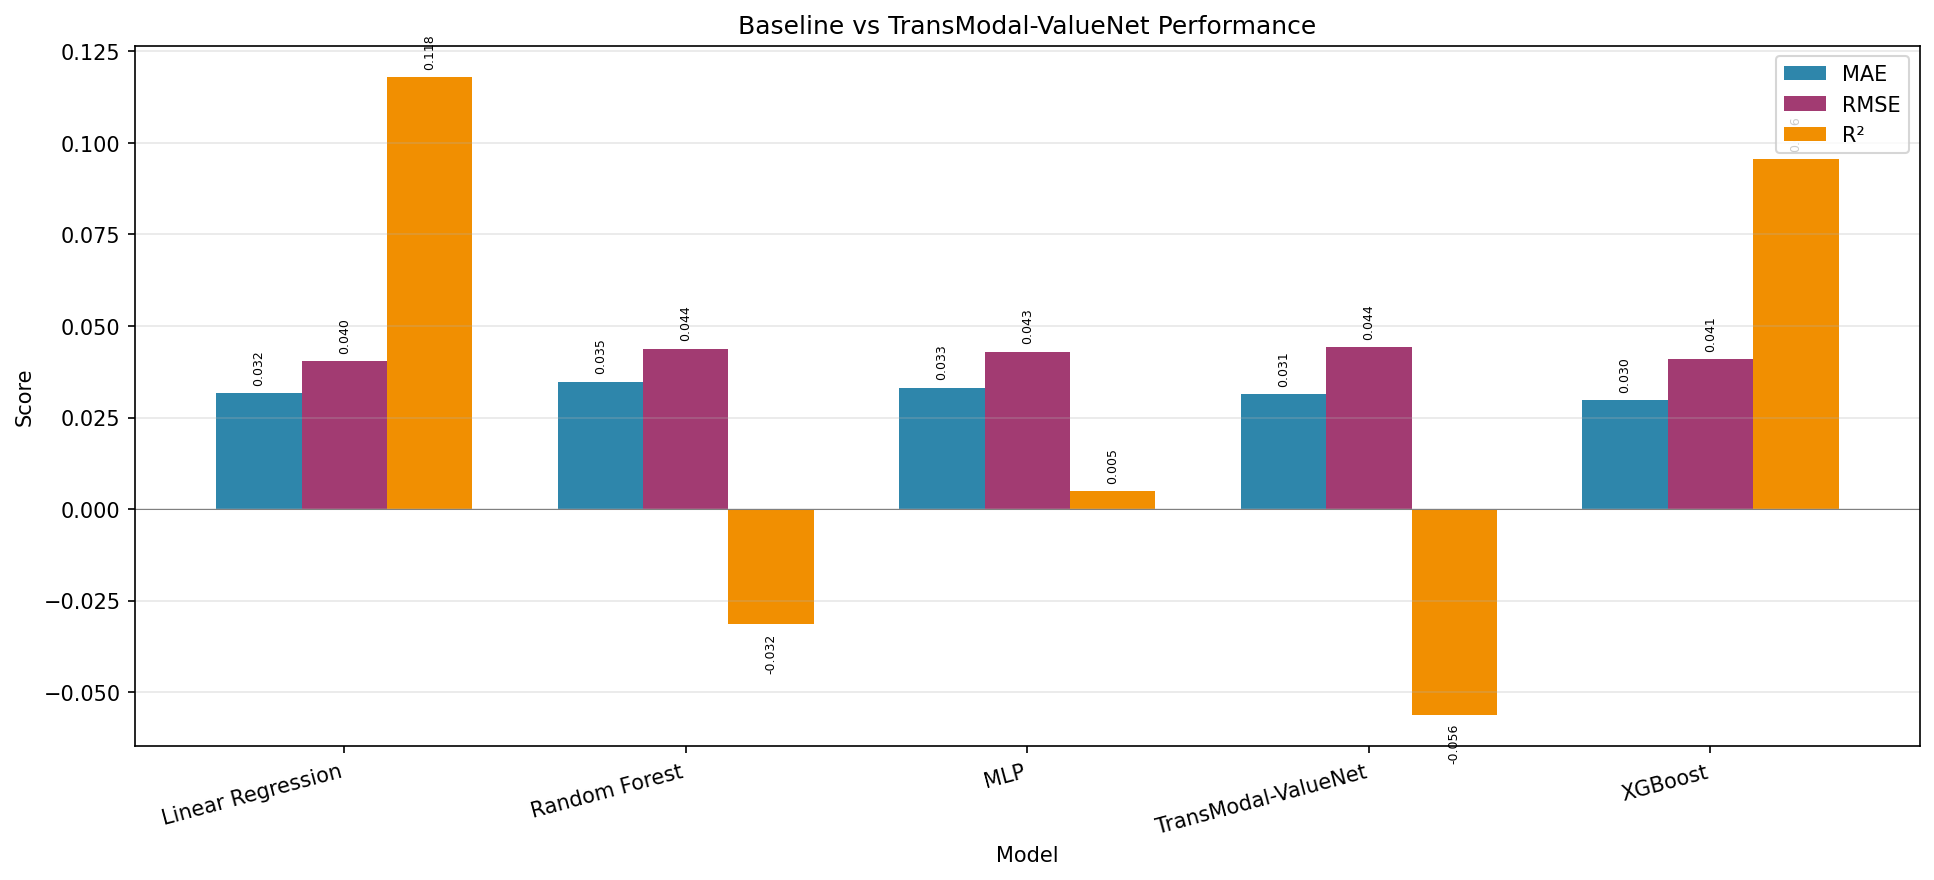
\includegraphics[width=0.85\columnwidth]{figures/baseline_comparison_bar.png}
  \caption{Performance comparison of all models across MAE, RMSE, and R\textsuperscript{2}. Classical tabular baselines remain strong under the full-year LMP setting, while TransModal-ValueNet is competitive in MAE but not dominant.}
  \label{fig:baseline_bar}
\end{figure}

\subsection{Seed Robustness of Valuation Baselines}

To verify that the baseline ranking is not caused by a favorable random seed, we rerun the stochastic valuation baselines with five seeds ($40$--$44$) while keeping the same chronological train/validation/test split. Table~\ref{tab:seed_robustness} reports mean and standard deviation across seeds. Linear Regression is deterministic under the fixed split, and XGBoost is effectively deterministic under the current configuration. MLP shows higher seed sensitivity, especially on R\textsuperscript{2}, while Random Forest remains consistently weaker on this test split.

\begin{table}[t!]
  \caption{Seed Robustness of Valuation Baselines (5 Seeds)}
  \label{tab:seed_robustness}
  \centering
  \begin{tabular}{lccc}
  \toprule
  \textbf{Model} & \textbf{MAE} $\downarrow$ & \textbf{RMSE} $\downarrow$ & \textbf{R\textsuperscript{2}} $\uparrow$ \\
  \midrule
  XGBoost & \textbf{0.0297} $\pm$ 0.0000 & 0.0410 $\pm$ 0.0000 & 0.0956 $\pm$ 0.0000 \\
  Linear Regression & 0.0317 $\pm$ 0.0000 & \textbf{0.0405} $\pm$ 0.0000 & \textbf{0.1179} $\pm$ 0.0000 \\
  MLP & 0.0318 $\pm$ 0.0022 & 0.0424 $\pm$ 0.0011 & 0.0318 $\pm$ 0.0508 \\
  Random Forest & 0.0352 $\pm$ 0.0004 & 0.0442 $\pm$ 0.0004 & $-$0.0521 $\pm$ 0.0179 \\
  \bottomrule
  \end{tabular}
\end{table}

These results reinforce the main conclusion from Table~\ref{tab:valuation_results}: the single-target proxy valuation task is well served by strong tabular baselines, and future gains from TransModal-ValueNet should be sought through stronger multi-target supervision, missing-modality robustness, or additional market/year validation rather than relying on a single seeded comparison.

\subsection{Ablation Study}

To examine whether the multimodal representation contributes beyond simple feature aggregation, we conduct both zero-shot interventional ablation and short fine-tuned ablation. The ablation metrics are averaged across the four proxy value dimensions and are therefore not directly comparable to the single-target baseline results in Table~\ref{tab:valuation_results}. In the zero-shot setting, removing generation features increases MAE from 0.0530 to 0.0730 ($+37.8\%$), and removing weather features increases MAE to 0.0572 ($+7.9\%$). Removing market or temporal features slightly improves zero-shot MAE, suggesting redundancy or instability before task-specific adaptation.

The short fine-tuned ablation shows clearer dependence on market, generation, and weather information. Removing market features increases MAE from 0.0545 to 0.0648 ($+19.0\%$), removing generation increases MAE to 0.0864 ($+58.6\%$), and removing weather increases MAE to 0.0769 ($+41.1\%$). These results support the use of heterogeneous power-system modalities, but they also show that the current proxy valuation task should be interpreted as an exploratory benchmark rather than a substitute for validation on real transaction prices.

\begin{figure}[t!]
  \centering
  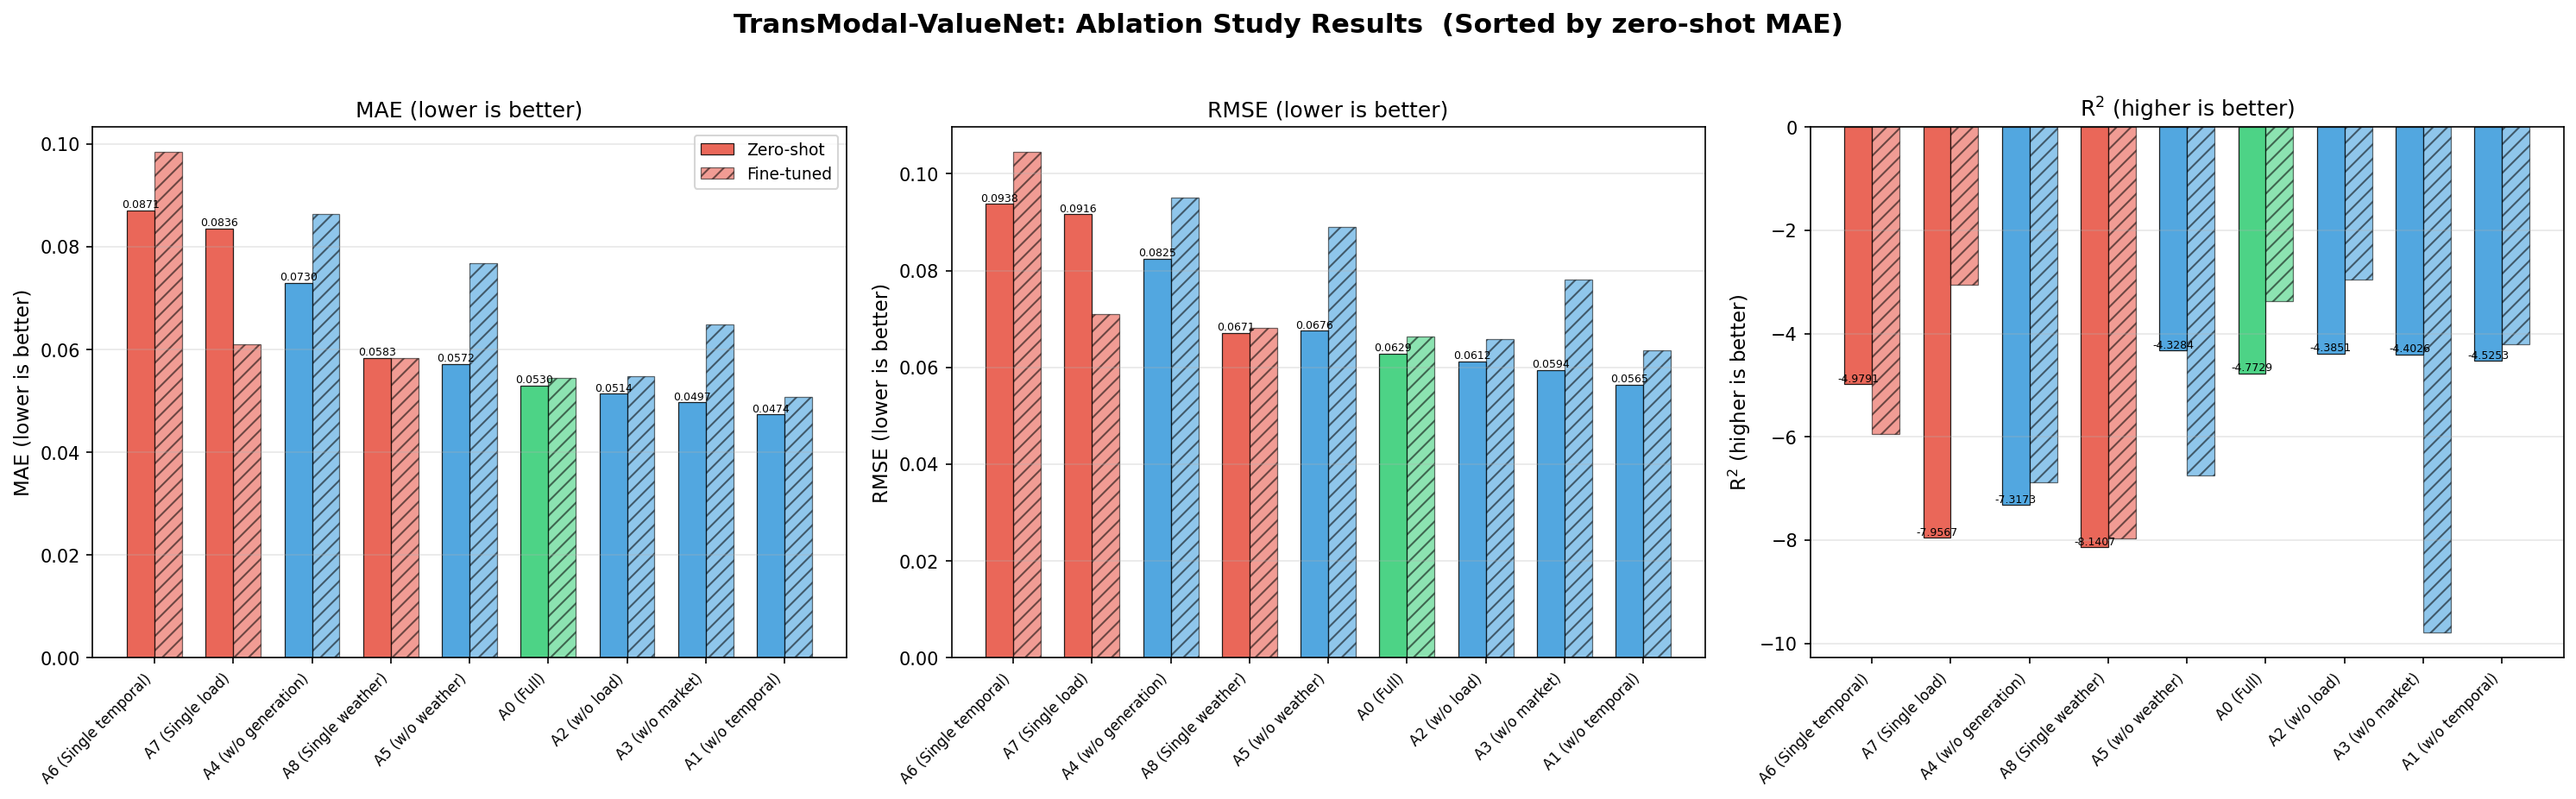
\includegraphics[width=0.98\columnwidth]{figures/ablation_results.png}
  \caption{Ablation study of TransModal-ValueNet under zero-shot and short fine-tuned settings. Metrics are averaged across four proxy value dimensions; lower MAE and RMSE and higher R\textsuperscript{2} are preferred.}
  \label{fig:ablation}
\end{figure}

\subsection{Market-Price Feature Robustness}

Because full-year LMP records are now available, we test whether the valuation results are overly dependent on market-price features. We rerun the December test-set evaluation after removing all four market-price columns (LMP, energy, congestion, and loss DAM). Fig.~\ref{fig:market_robustness} reports MAE for Linear Regression, Random Forest, and XGBoost under the full-feature and price-removed settings.

The results show mixed but informative behavior. Linear Regression degrades slightly when market-price features are removed (MAE 0.0317 to 0.0321, $+1.2\%$), Random Forest degrades modestly (0.0348 to 0.0369, $+6.1\%$), while XGBoost is more sensitive (0.0321 to 0.0407, $+26.5\%$). Therefore, the reported valuation signal is not solely driven by price features, but nonlinear tree boosting exploits market-price covariates more strongly than the other tested baselines.

\begin{figure}[t!]
  \centering
  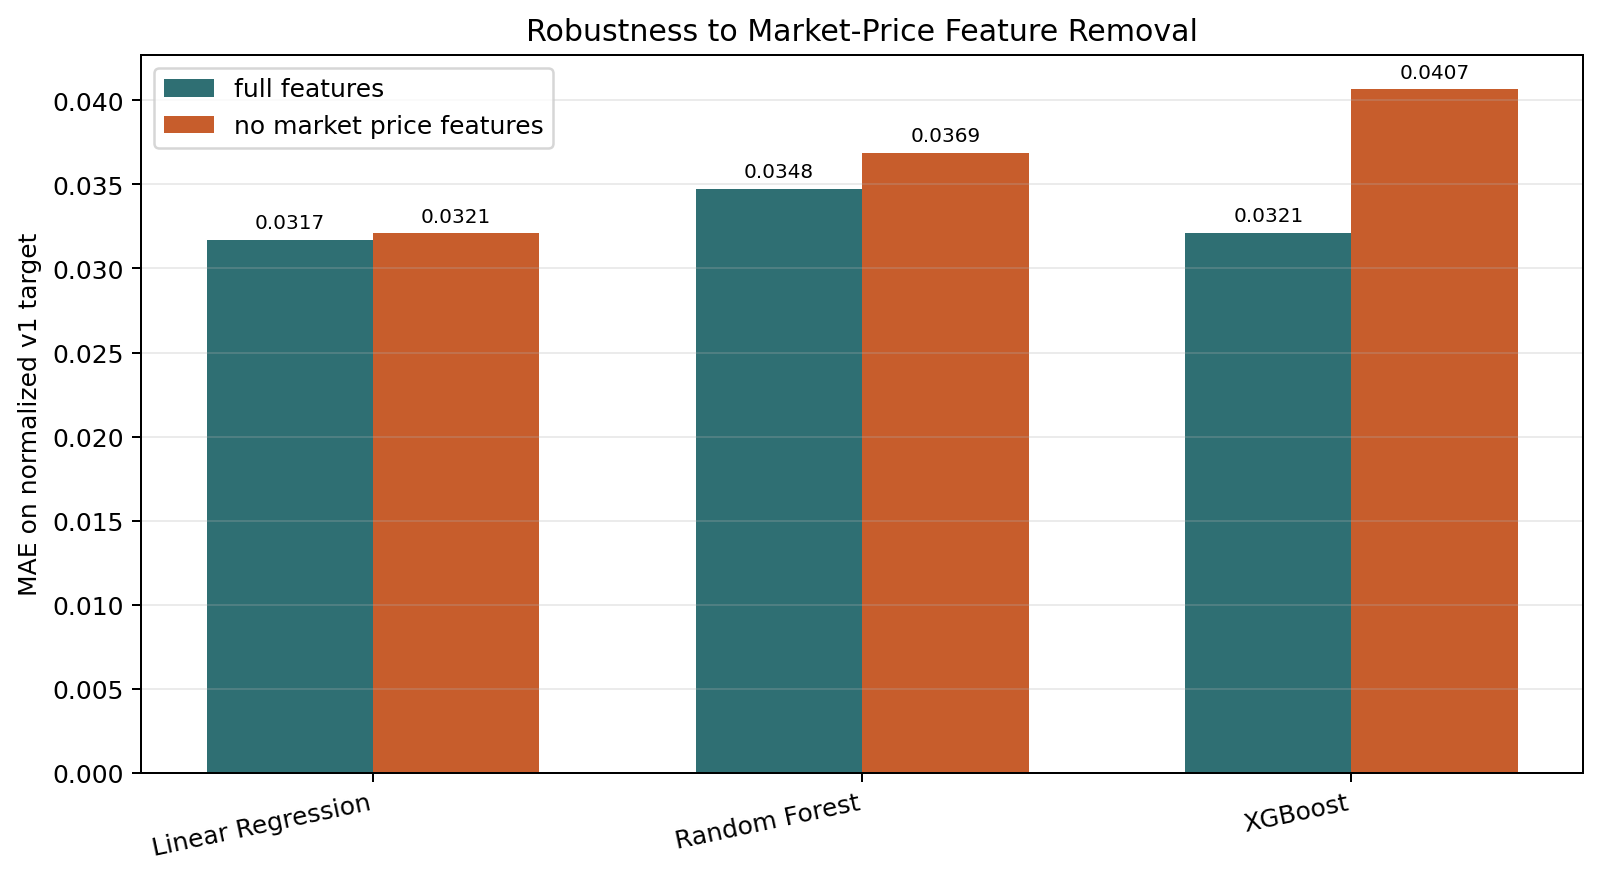
\includegraphics[width=0.95\columnwidth]{figures/market_feature_robustness.png}
  \caption{Robustness to market-price feature removal on the December test set. Removing LMP-related features has limited effect on Linear Regression and Random Forest, but degrades XGBoost, indicating useful but not exclusively determining price-feature information.}
  \label{fig:market_robustness}
\end{figure}

\subsection{DRL-Based Trading Performance}

Table~\ref{tab:trading_results} summarizes the saved SAC agent's performance on the 12-day (3,456 step) test set. The SAC policy achieves 3.41$\times$ higher average reward (13,436 vs.\ 3,942) and total reward (46.4M vs.\ 13.6M) compared to the random policy. The deal rate improves from 83.62\% to 90.13\%, indicating that the learned policy facilitates successful trades in a larger fraction of market conditions.

\begin{table}[t!]
  \caption{P2P Trading Performance: SAC vs.\ Random Policy}
  \label{tab:trading_results}
  \centering
  \begin{tabular}{lcc}
  \toprule
  \textbf{Metric} & \textbf{SAC (Ours)} & \textbf{Random} \\
  \midrule
  Average reward & 13,436 & 3,942 \\
  Total reward & 46,433,648 & 13,623,923 \\
  Average clearing price & \$252.48 & \$256.59 \\
  Deal rate (nonzero volume) & 90.13\% & 83.62\% \\
  \bottomrule
  \end{tabular}
\end{table}

To assess training robustness, we additionally retrain SAC with three random seeds (40, 41, and 42), each for 30,000 timesteps, and compare against random policies evaluated with matching seeds. Table~\ref{tab:sac_seed} shows that SAC retains a large reward advantage despite noticeable policy-level reward variation. The mean average reward is 12,639 $\pm$ 2,063 per step, compared with 3,940 $\pm$ 9 for random matching; the mean total reward advantage is approximately 3.21$\times$. The deal rate is stable at 90.13\% across all SAC seeds.

\begin{table}[t!]
  \caption{SAC Seed Robustness on P2P Trading (3 Seeds)}
  \label{tab:sac_seed}
  \centering
  \begin{tabular}{lcc}
  \toprule
  \textbf{Metric} & \textbf{SAC} & \textbf{Random} \\
  \midrule
  Average reward & 12,639 $\pm$ 2,063 & 3,940 $\pm$ 9 \\
  Total reward & 43.68M $\pm$ 7.13M & 13.62M $\pm$ 0.03M \\
  Average clearing price & \$251.06 $\pm$ 16.92 & \$256.71 $\pm$ 0.53 \\
  Deal rate & 90.13\% $\pm$ 0.00\% & 83.27\% $\pm$ 0.48\% \\
  \bottomrule
  \end{tabular}
\end{table}

Fig.~\ref{fig:trading_price} shows the time-series comparison of clearing prices. The SAC agent maintains prices closer to the grid buy price (\$300/MWh) during high-demand periods and closer to the feed-in tariff (\$50/MWh) during surplus periods, indicating more economically rational market operation compared to random actions that frequently select sub-optimal prices.

\begin{figure}[t!]
  \centering
  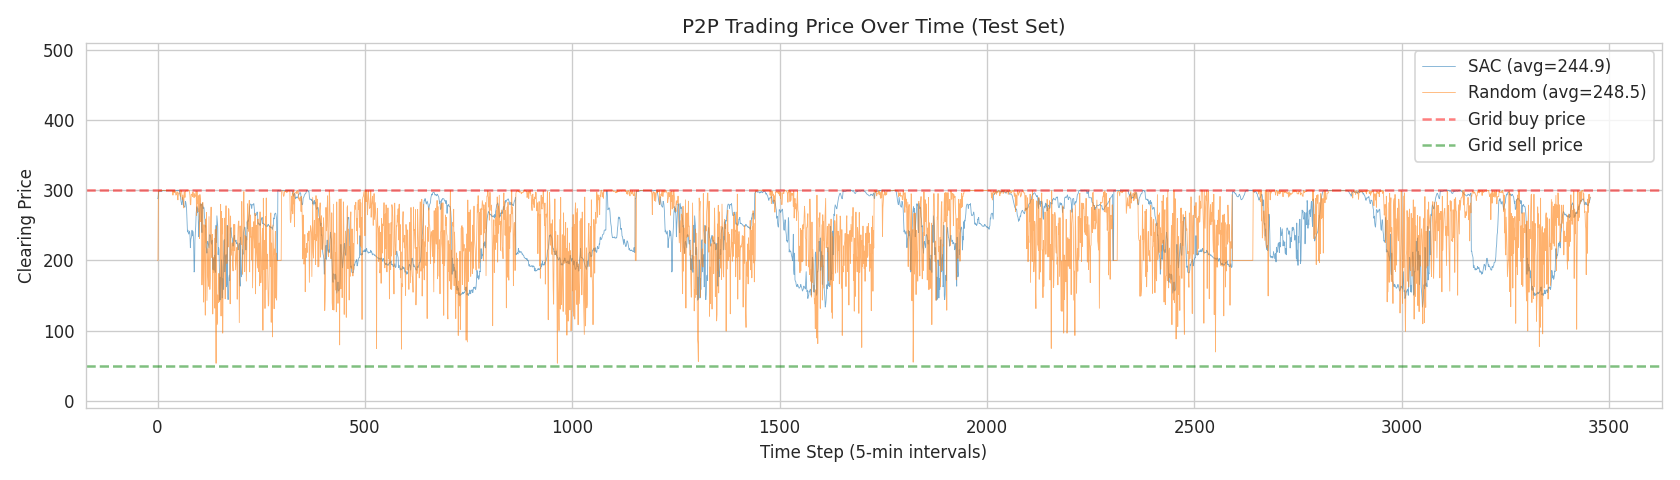
\includegraphics[width=0.85\columnwidth]{figures/drl_trading_price.png}
  \caption{P2P trading clearing price comparison. The SAC agent (orange) shows more structured pricing behavior compared to the random policy (blue), maintaining prices within economically meaningful bounds.}
  \label{fig:trading_price}
\end{figure}

Fig.~\ref{fig:cum_reward} shows the cumulative reward trajectories. The SAC policy's cumulative reward diverges steadily from random, demonstrating consistent value generation from learned trading strategies.

\begin{figure}[t!]
  \centering
  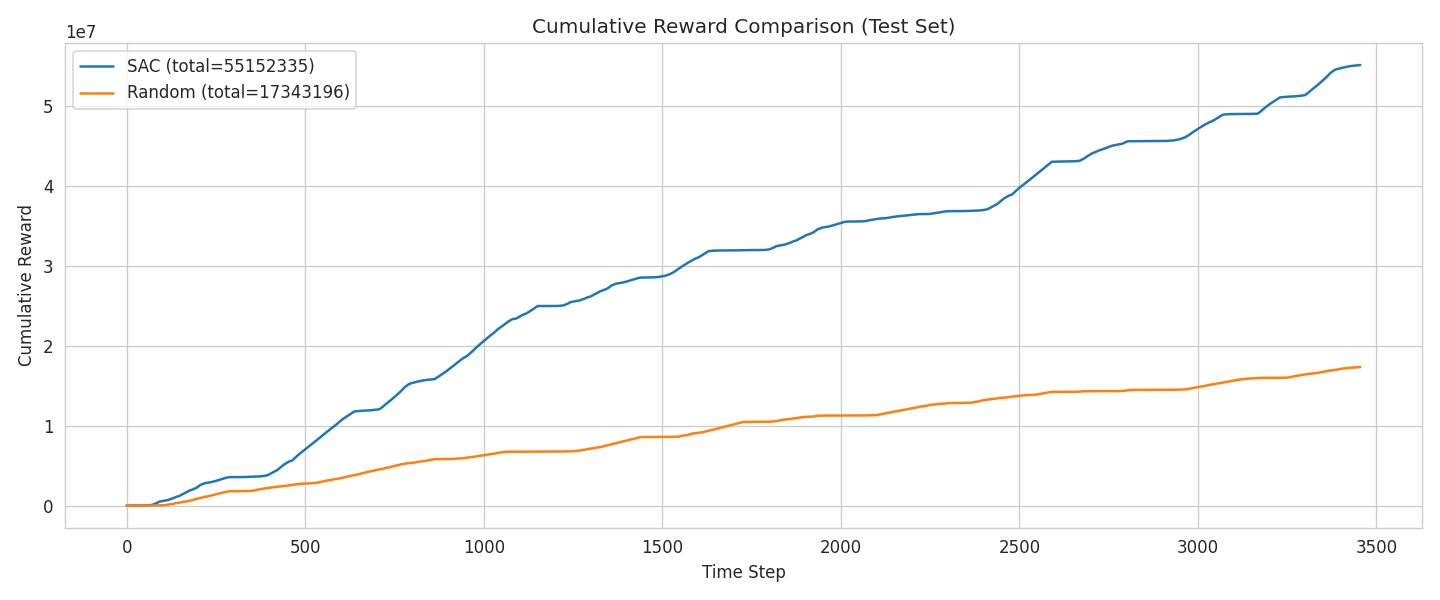
\includegraphics[width=0.85\columnwidth]{figures/drl_cumulative_reward.png}
  \caption{Cumulative reward comparison on the test set. SAC consistently outperforms the random baseline, with the gap widening over time.}
  \label{fig:cum_reward}
\end{figure}

\subsection{Privacy-Utility Optimization}

Fig.~\ref{fig:privacy_tradeoff} presents the privacy-utility trade-off curves for both smoothed adaptive and uniform DP mechanisms across $\varepsilon \in \{0.1, 0.5, 1.0, 2.0, 5.0, 10.0\}$. The non-private Random Forest reference obtains R\textsuperscript{2} = 0.882 on the LMP target. Key findings:

\begin{itemize}
  \item At $\varepsilon = 10$ (moderate privacy), uniform DP preserves 25.9\% of the non-private value, while the current smoothed adaptive allocation preserves 16.9\%, a 9.0 percentage point disadvantage.
  \item At $\varepsilon \leq 2.0$, both mechanisms preserve almost no predictive utility under the current Gaussian-noise calibration, indicating that strong privacy settings require either additional utility-preserving preprocessing or a different task formulation.
  \item At $\varepsilon = 0.1$ (strong privacy), both mechanisms approach zero utility, consistent with the fundamental limits of DP under stringent privacy guarantees.
\end{itemize}

This negative result indicates that feature-importance tilting can amplify noise sensitivity when the target is volatile full-year LMP. Fig.~\ref{fig:epsilon_alloc} visualizes the allocation difference at $\varepsilon_{\text{total}} = 2.0$, where the smoothed adaptive mechanism keeps a 75\% uniform allocation floor and uses a 25\% importance tilt. The result suggests that future adaptive DP designs should select or clip group budgets using validation performance rather than relying only on static feature importance.

\begin{figure}[t!]
  \centering
  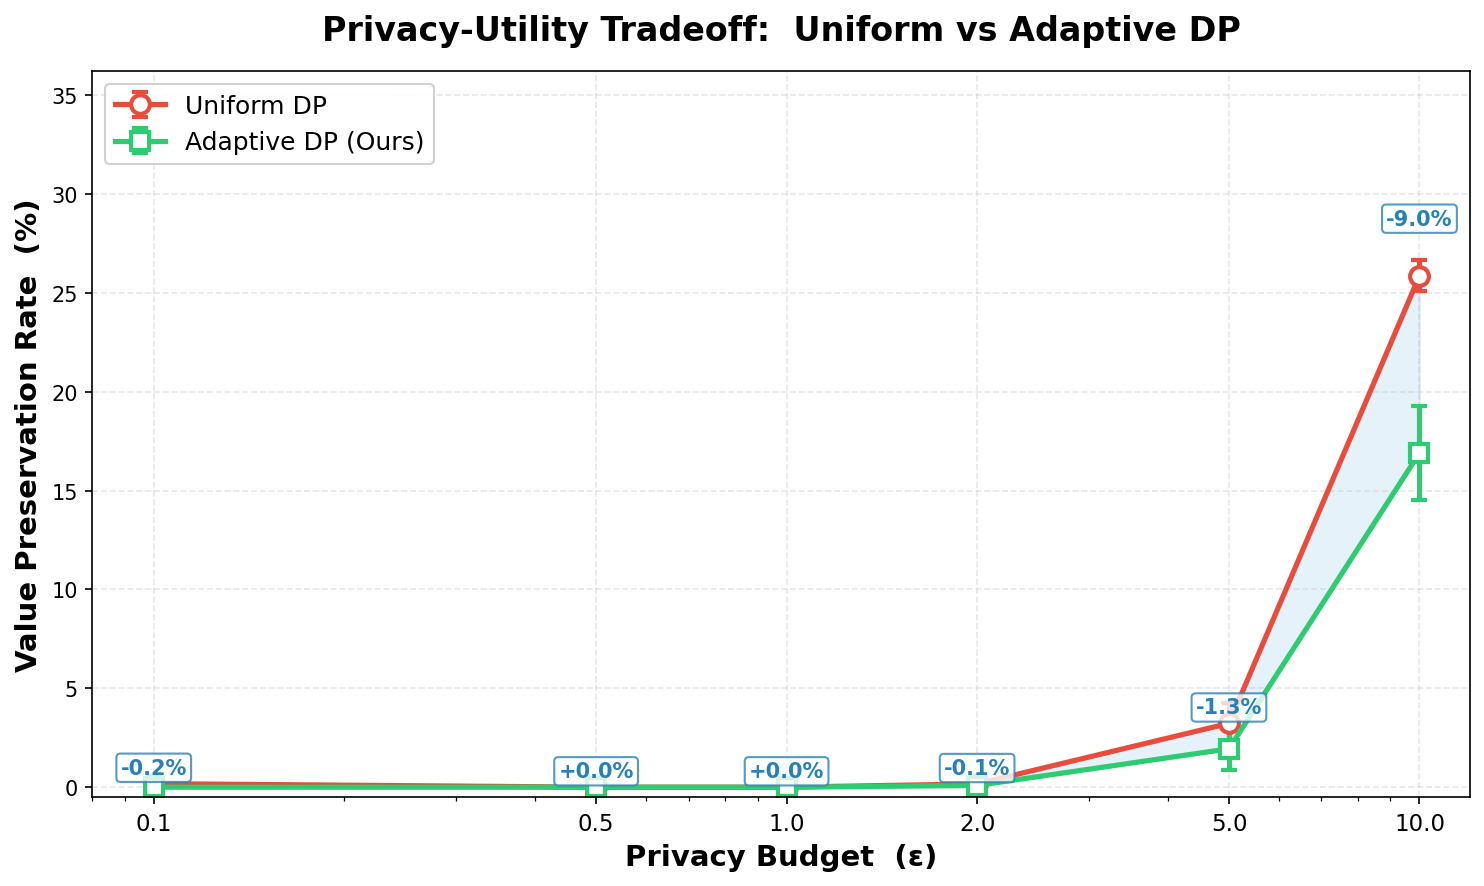
\includegraphics[width=0.85\columnwidth]{figures/privacy_utility_tradeoff.png}
  \caption{Privacy-utility trade-off under full-year LMP. Uniform DP outperforms the current smoothed adaptive allocation at $\varepsilon = 10$, showing that feature-importance-based allocation requires additional validation-aware safeguards.}
  \label{fig:privacy_tradeoff}
\end{figure}

\begin{figure}[t!]
  \centering
  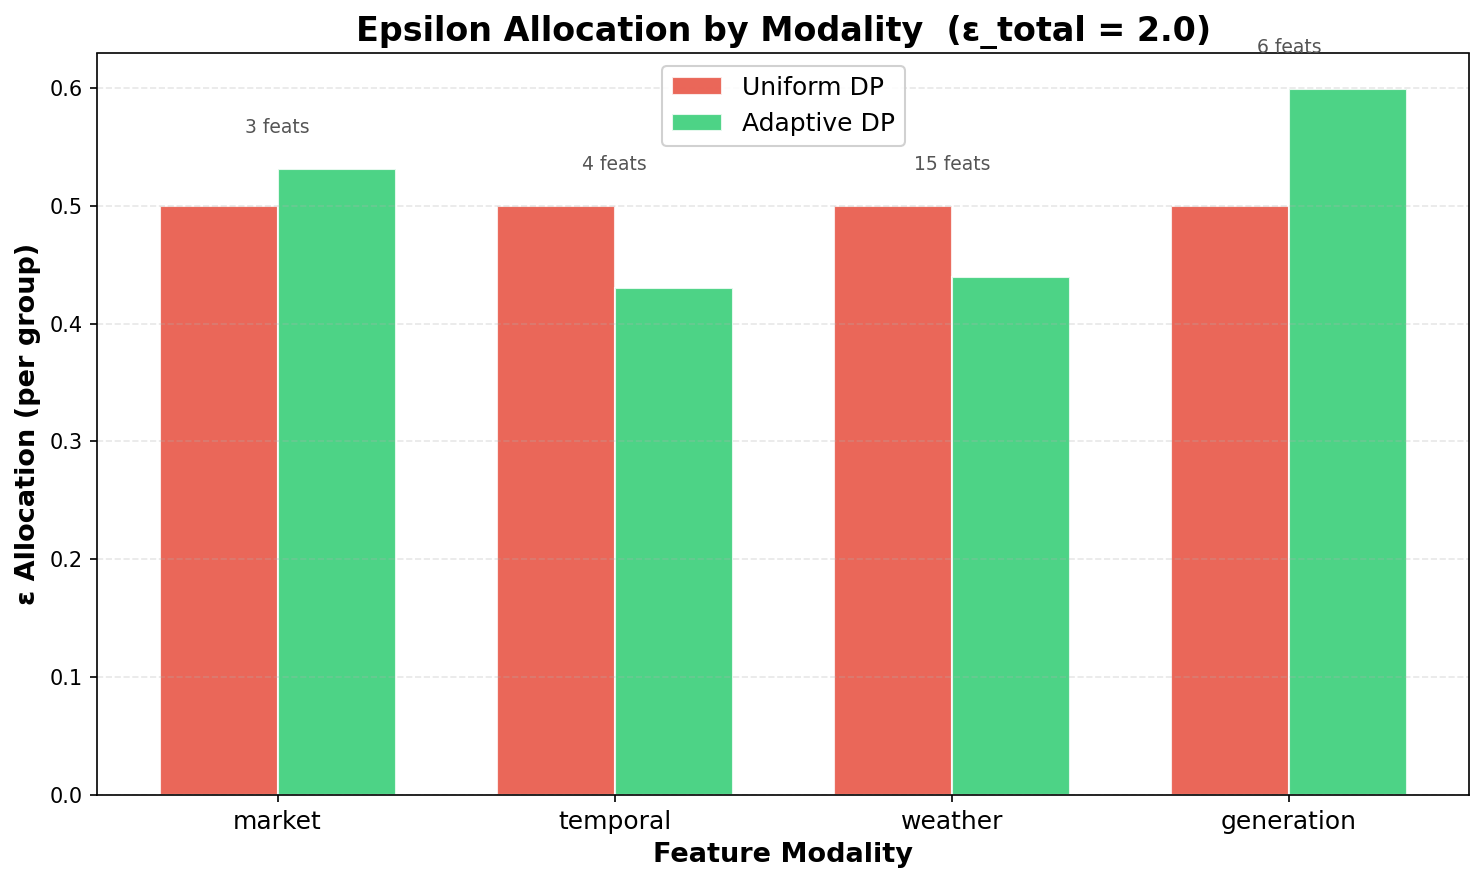
\includegraphics[width=0.85\columnwidth]{figures/epsilon_allocation.png}
  \caption{Epsilon budget allocation by modality at $\varepsilon_{\text{total}} = 2.0$. The smoothed adaptive mechanism uses a 75\% uniform floor and a 25\% feature-importance tilt across active modality groups.}
  \label{fig:epsilon_alloc}
\end{figure}

\subsection{Multimodal Feature Analysis}

Fig.~\ref{fig:feature_importance} displays the Random Forest-based feature importance scores for the LMP target after removing direct price leakage columns. The group-level shares are generation (44.8\%), load/market (31.3\%), weather (12.9\%), and temporal (11.0\%). Top-ranked features include solar generation, day-ahead and hour-ahead demand forecasts, month, biomass generation, system demand, small hydro generation, and selected weather variables. This cross-modality distribution supports multimodal feature construction, while also showing that generation and load signals are especially important for this target.

\begin{figure}[t!]
  \centering
  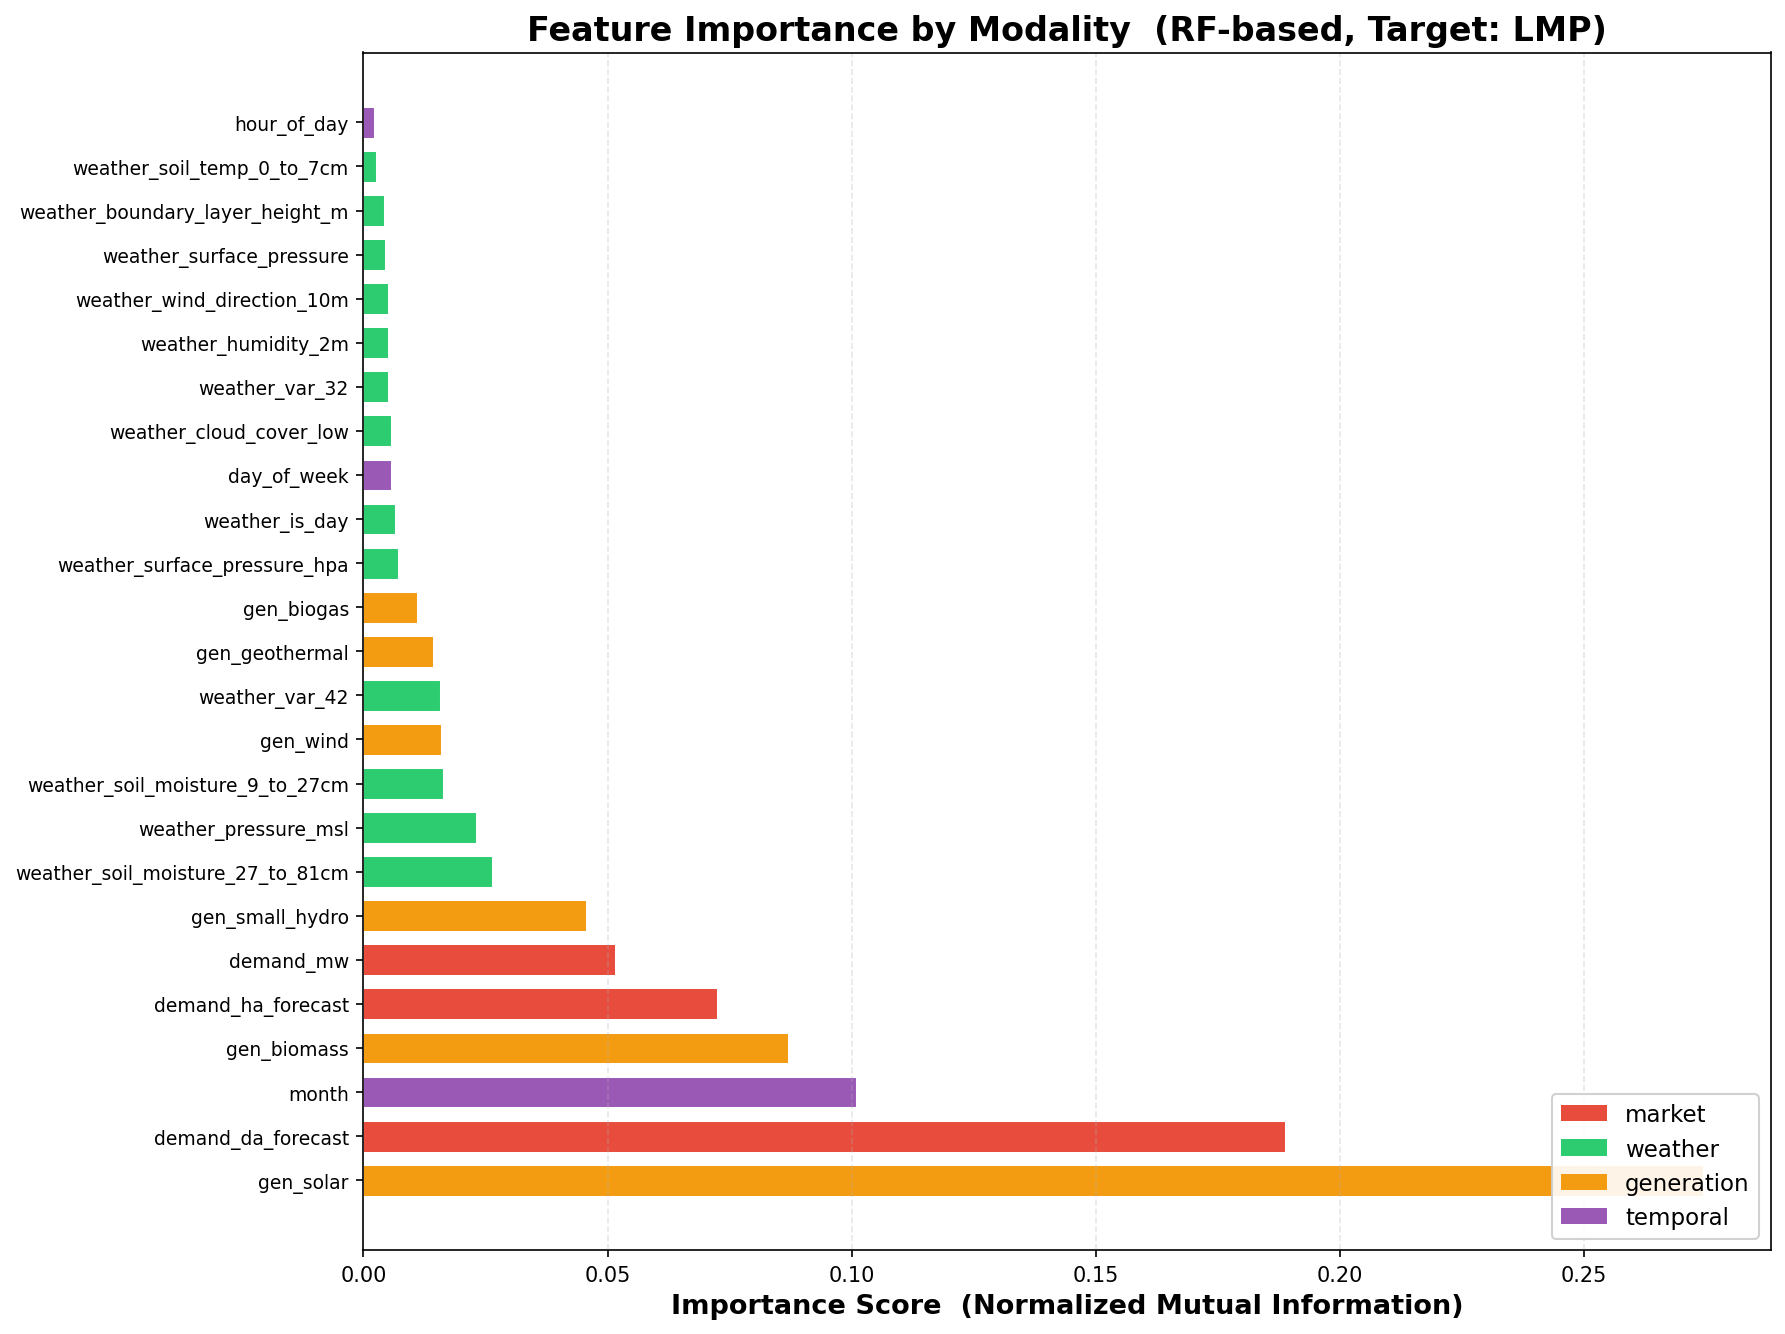
\includegraphics[width=0.85\columnwidth]{figures/feature_importance.png}
  \caption{Feature importance scores (RF-based, target: LMP, direct price columns removed). The top 25 features span generation, load/market, weather, and temporal modalities.}
  \label{fig:feature_importance}
\end{figure}

Fig.~\ref{fig:correlation} presents the correlation heatmap, revealing strong inter-modality correlations (e.g., temperature vs.\ load, cloud cover vs.\ solar generation) that the cross-attention mechanism can exploit.

\begin{figure}[t!]
  \centering%
  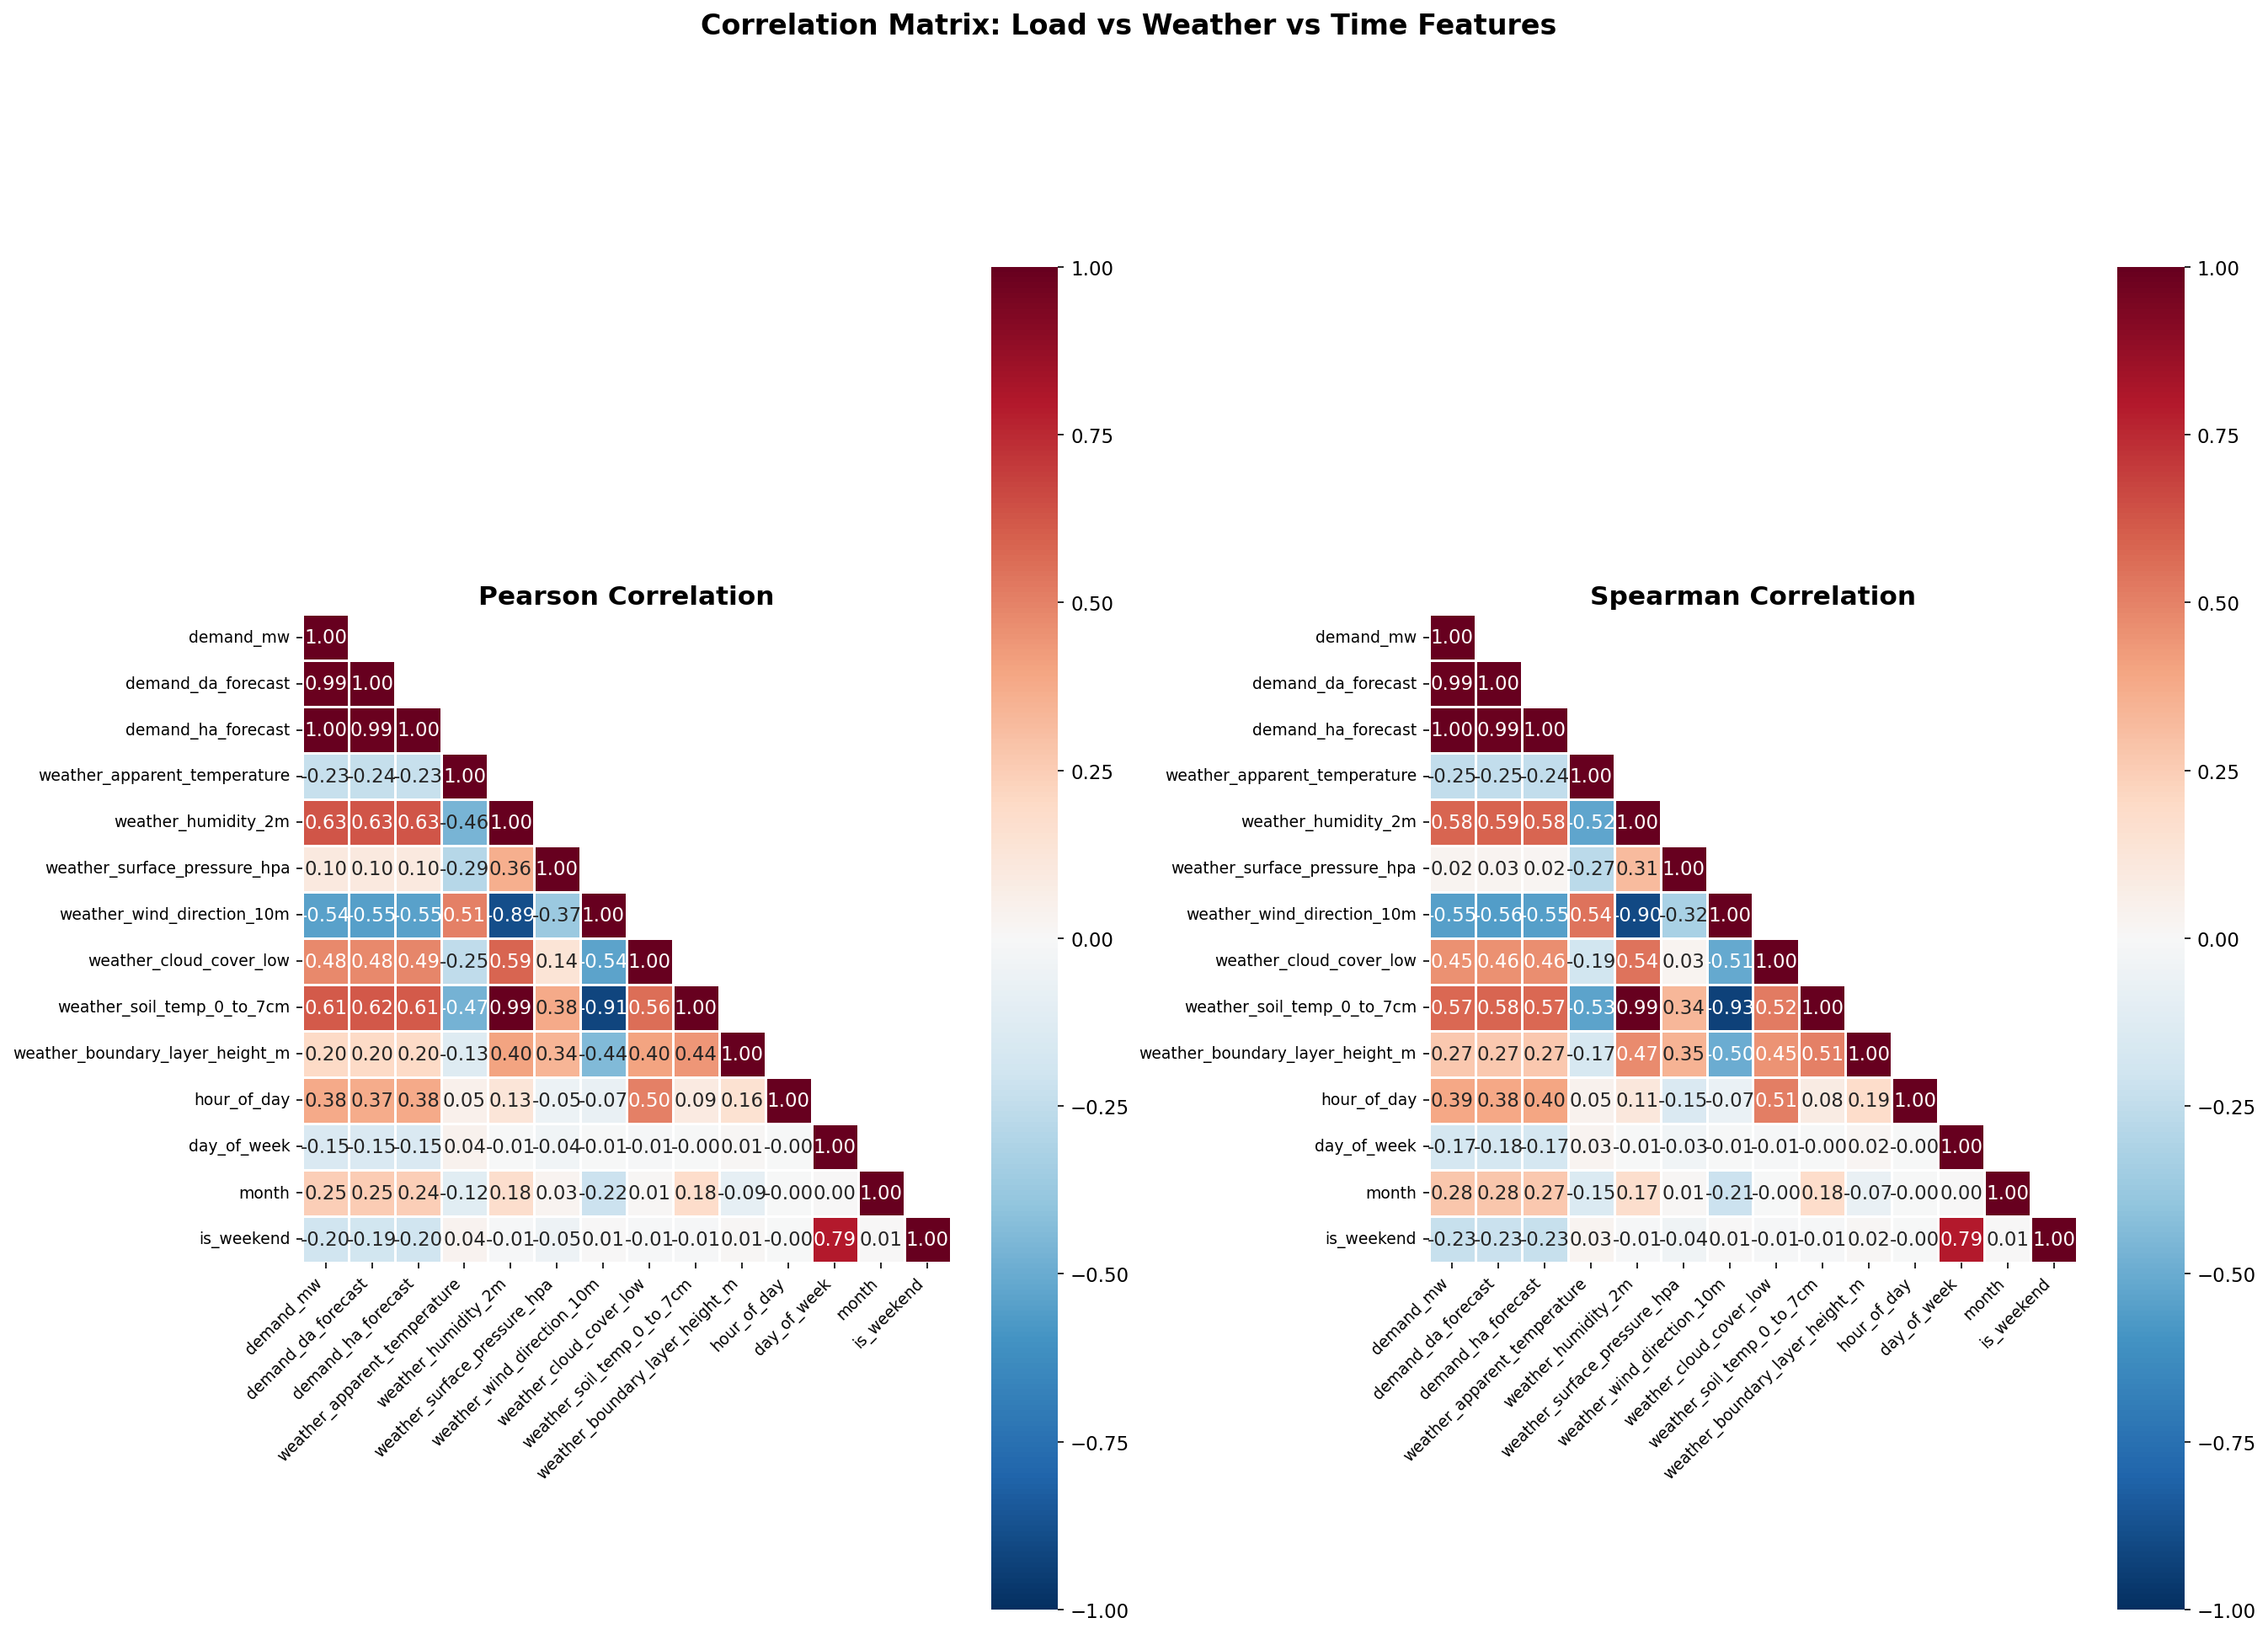
\includegraphics[width=0.85\columnwidth]{figures/correlation_heatmap.png}
  \caption{Correlation heatmap of multimodal features. Significant cross-modality correlations (e.g., weather $\leftrightarrow$ load, weather $\leftrightarrow$ renewable generation) motivate the use of cross-attention fusion.}
  \label{fig:correlation}
\end{figure}

\subsection{Training Dynamics}

Fig.~\ref{fig:training_loss} shows the pre-training and fine-tuning loss curves. The masked autoencoder pre-training converges rapidly within the early epochs, suggesting that cross-modal reconstruction provides a useful learning signal. Fine-tuning validation loss reaches its best value early under the full-year LMP setting, and early stopping (patience~5) prevents further overfitting.

\begin{figure}[t!]
  \centering
  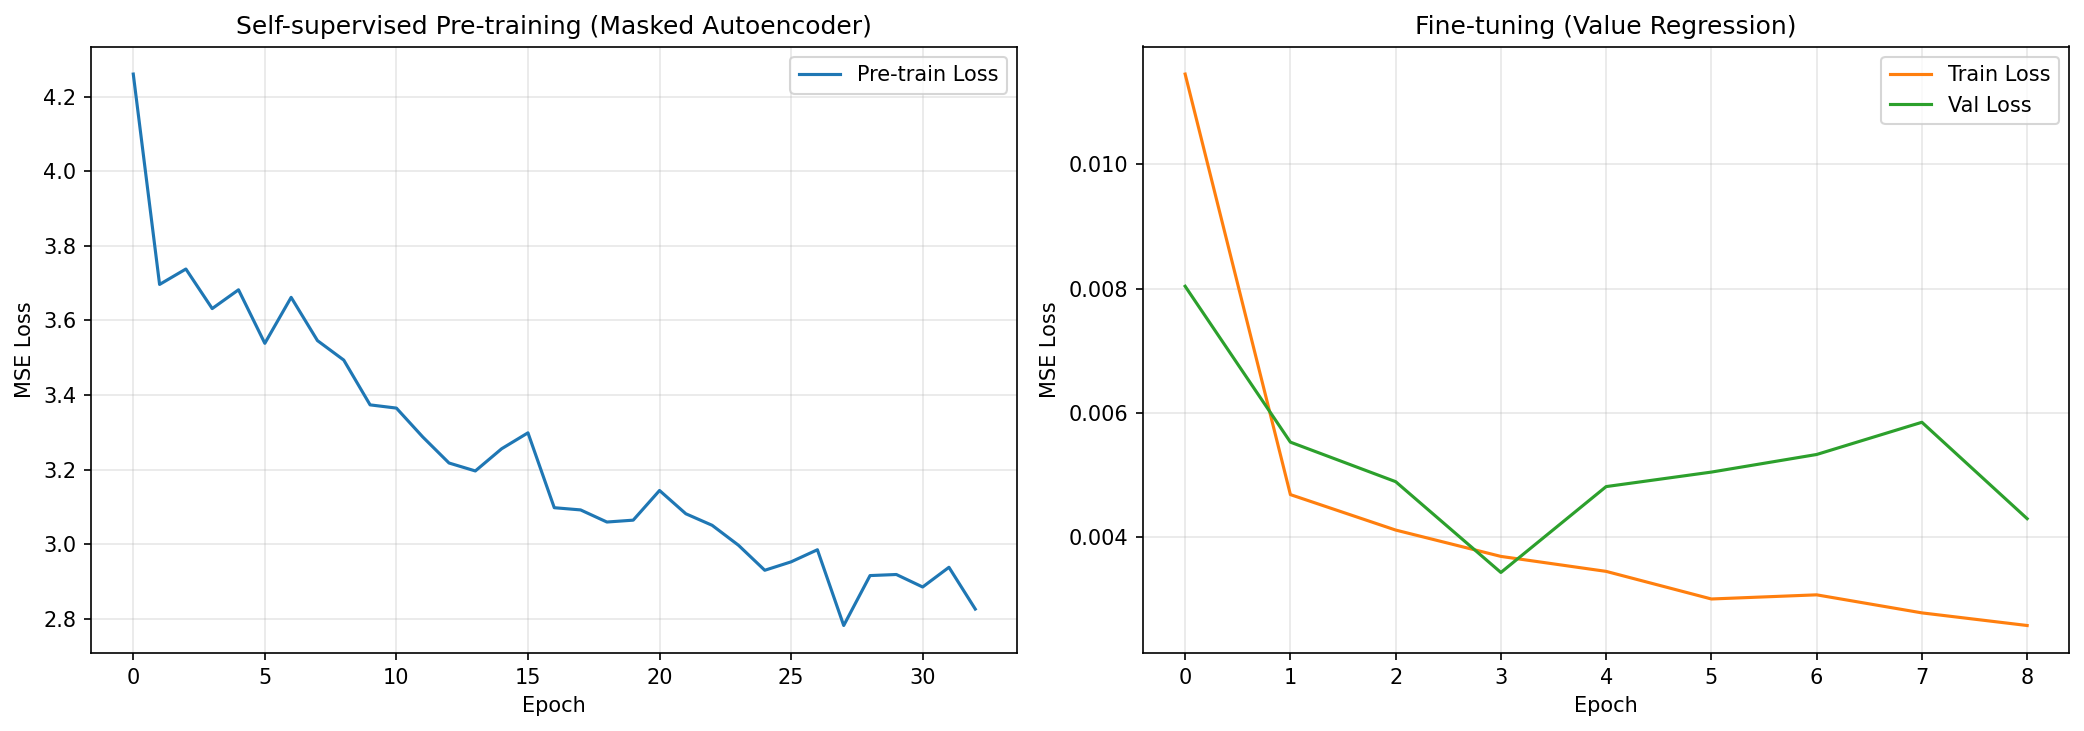
\includegraphics[width=0.85\columnwidth]{figures/training_loss.png}
  \caption{Training loss curves. Left: masked autoencoder pre-training converges within 10 epochs. Right: value regression fine-tuning with early stopping prevents overfitting.}
  \label{fig:training_loss}
\end{figure}

\subsection{Discussion and Key Insights}

\textbf{Framework-level value proposition:} The main empirical value of the proposed system is the integration of data valuation, buyer-query interpretation, trading optimization, and privacy-utility analysis in one reproducible workflow. This is important for power data markets because a usable platform must decide not only how valuable a dataset is, but also how it should be matched, traded, and released under privacy constraints.

\textbf{Why valuation performance is mixed:} The full-year LMP update creates a harder valuation setting than the earlier partial-price package. Classical tabular methods remain strong on the single-target proxy label: XGBoost obtains the lowest MAE and Linear Regression obtains the highest R\textsuperscript{2}. TransModal-ValueNet is still useful as a multimodal representation model, but the current training recipe does not yet deliver consistent gains over strong tabular baselines.

\textbf{The value of self-supervised pre-training:} The MAE pre-training phase forces the model to learn cross-modal dependencies---e.g., the relationship between cloud cover (weather) and solar generation (generation), or between temperature (weather) and demand (load). These learned representations provide a strong initialization for the downstream valuation task.

\textbf{DRL for P2P trading:} The SAC agent learns trading strategies that exploit temporal patterns in microgrid net loads---e.g., anticipating morning solar ramps and evening load peaks---which a random policy cannot capture. The 90.13\% deal rate indicates that the agent successfully identifies mutually beneficial trading opportunities in most market conditions.

\textbf{Privacy-utility frontier:} The privacy experiment provides a useful cautionary result. Under full-year LMP, the current feature-importance-guided allocation underperforms uniform DP at $\varepsilon=10$, suggesting that adaptive privacy allocation must be selected using validation-aware utility criteria rather than static importance alone.

\textbf{Limitations:} (1) The current study uses a single geographic region (California CAISO) and a single year (2024); generalizability to other markets requires validation. (2) The value labels are derived from proxy heuristics rather than ground-truth transaction data. (3) TransModal-ValueNet does not yet outperform all tabular baselines on the full-year single-target valuation task, and the multi-target ablation shows instability in explained variance. (4) The current adaptive DP allocation underperforms uniform DP under full-year LMP, so privacy-budget optimization remains an open component. (5) The privacy analysis assumes the attacker has no auxiliary information; real-world adversaries may be more capable.

\section{Conclusion and Future Work}
\label{sec:conclusion}

This paper presented an end-to-end multimodal AI framework for power data asset valuation and trading. We introduced three executable modules---TransModal-ValueNet for cross-attention-based proxy valuation, a natural-language-assisted DRL engine for intelligent data matching, and a heterogeneous differential privacy stress-test module---and validated each on datasets from CAISO, Open-Meteo, and P2P microgrid environments. The experimental results show strong DRL trading performance, mixed but informative valuation performance where classical tabular baselines remain competitive, and a privacy stress test in which uniform DP outperforms the current smoothed adaptive allocation under full-year LMP. The main contribution is therefore a reproducible applied workflow and empirical benchmark for power data asset markets, not a claim that every proposed component is already optimal.

Several directions for future research are identified:

\begin{enumerate}
  \item \textbf{Geographic and Temporal Extension}: Validation on additional ISO markets (PJM, ERCOT, MISO, NYISO) across multiple years (2020--2025) to establish cross-market generalizability.

  \item \textbf{Multi-Agent Trading}: Extension to multi-agent reinforcement learning (MADDPG, MAPPO) where each market participant learns an independent bidding strategy, enabling simulation of strategic interactions and market power analysis.

  \item \textbf{Federated Valuation}: Integration of federated learning with the TransModal-ValueNet architecture to enable privacy-preserving collaborative valuation across multiple data owners without centralizing raw data \cite{b33}.

  \item \textbf{Domain-Specific Query Understanding}: Fine-tuning domain-specific language models on power market text corpora (EIA reports, ISO announcements, regulatory filings) to improve query understanding and enable automated market commentary generation.

  \item \textbf{Live Deployment}: Implementation of a prototype platform with real-time data ingestion, model inference, and smart contract settlement on a blockchain testnet, evaluating end-to-end latency and throughput.
\end{enumerate}

\appendices

We include supplementary material comprising detailed hyperparameter configurations and additional experimental results in an online repository. The final public repository URL will be inserted after author and repository verification.

\section*{Acknowledgment}

The authors thank the California Independent System Operator (CAISO) for providing open access to market data, and the Open-Meteo project for freely accessible meteorological archives. The P2P microgrid dataset provided by Mendeley Data is gratefully acknowledged.

\subsection*{Data and Code Availability}
All code used in this study will be made available in a public repository after author and repository verification. The reproducibility package should include the cleaned fused dataset and document the full-year LMP source, local-time alignment, and daylight-saving-hour filling step. Datasets are publicly accessible: CAISO data through CAISO public market-data portals, Open-Meteo data at \texttt{https://open-meteo.com/}, and P2P microgrid data at Mendeley Data (DOI: 10.17632/s7dg7wfzsz.2).


\begin{thebibliography}{00}

\bibitem{b1} State Council of the People's Republic of China, ``Opinions on building a more complete factor market allocation system and mechanism,'' 2020. [Online]. Available: http://www.gov.cn/zhengce/2020-04/09/content_5500622.htm

\bibitem{b2} C. Li, D. Y. Li, G. Miklau, and D. Suciu, ``A theory of pricing private data,'' \emph{ACM Trans. Database Syst.}, vol. 39, no. 4, Art. no. 34, 2014.

\bibitem{b3} A. Vaswani \emph{et al.}, ``Attention is all you need,'' in \emph{Proc. NeurIPS}, 2017, pp. 5998--6008.

\bibitem{b4} J. Achiam \emph{et al.}, ``GPT-4 technical report,'' arXiv preprint arXiv:2303.08774, 2023.

\bibitem{b5} T. Haarnoja, A. Zhou, P. Abbeel, and S. Levine, ``Soft actor-critic: Off-policy maximum entropy deep reinforcement learning with a stochastic actor,'' in \emph{Proc. ICML}, 2018, pp. 1861--1870.

\bibitem{b6} P. Koutris, P. Upadhyaya, M. Balazinska, B. Howe, and D. Suciu, ``Query-based data pricing,'' in \emph{Proc. ACM SIGMOD-SIGACT-SIGART Symp. Principles of Database Systems (PODS)}, 2012, pp. 167--178.

\bibitem{b7} A. Ghorbani and J. Zou, ``Data Shapley: Equitable valuation of data for machine learning,'' in \emph{Proc. ICML}, 2019, pp. 2242--2251.

\bibitem{b8} Y. Kwon and J. Zou, ``Beta Shapley: A unified and noise-reduced data valuation framework for machine learning,'' in \emph{Proc. AISTATS}, 2022, pp. 8780--8802.

\bibitem{b9} J. Yoon, S. Arik, and T. Pfister, ``Data valuation using reinforcement learning,'' in \emph{Proc. ICML}, 2020, pp. 10842--10851.

\bibitem{b10} W. Tushar \emph{et al.}, ``Peer-to-peer trading in electricity networks: An overview,'' \emph{Appl. Energy}, vol. 220, pp. 1--18, 2018.

\bibitem{b11} E. Mengelkamp, B. Notheisen, C. Beer, D. Dauer, and C. Weinhardt, ``Designing microgrid energy markets: A case study: The Brooklyn Microgrid,'' \emph{Appl. Energy}, vol. 210, pp. 870--880, 2018.

\bibitem{b12} J. Kang, R. Yu, X. Huang, S. Maharjan, Y. Zhang, and E. Hossain, ``Enabling localized peer-to-peer electricity trading among plug-in hybrid electric vehicles using consortium blockchains,'' \emph{IEEE Trans. Ind. Informat.}, vol. 13, no. 6, pp. 3154--3164, 2017.

\bibitem{b13} M. Andoni \emph{et al.}, ``Blockchain technology in the energy sector: A systematic review of challenges and opportunities,'' \emph{Renew. Sustain. Energy Rev.}, vol. 100, pp. 143--174, 2019.

\bibitem{b14} B. Lim, S. \"{O}. Arik, N. Loeff, and T. Pfister, ``Temporal Fusion Transformers for interpretable multi-horizon time series forecasting,'' \emph{Int. J. Forecasting}, vol. 37, no. 4, pp. 1748--1764, 2021.

\bibitem{b15} K. Rasul \emph{et al.}, ``Lag-Llama: Towards foundation models for probabilistic time series forecasting,'' arXiv preprint arXiv:2310.08278, 2023.

\bibitem{b16} J. Lago, G. Marcjasz, B. De Schutter, and R. Weron, ``Forecasting day-ahead electricity prices: A review of state-of-the-art algorithms, best practices and an open-access benchmark,'' \emph{Appl. Energy}, vol. 293, Art. no. 116983, 2021.

\bibitem{b17} R. Lowe \emph{et al.}, ``Multi-agent actor-critic for mixed cooperative-competitive environments,'' in \emph{Proc. NeurIPS}, 2017, pp. 6379--6390.

\bibitem{b18} Y. Nie, N. H. Nguyen, P. Sinthong, and J. Kalagnanam, ``A time series is worth 64 words: Long-term forecasting with Transformers,'' in \emph{Proc. ICLR}, 2023.

\bibitem{b19} G. \'{A}cs and C. Castelluccia, ``I have a DREAM! (DiffeRentially privatE smArt Metering),'' in \emph{Proc. Information Hiding}, 2011, pp. 118--132.

\bibitem{b20} F. Fioretto, T. W. K. Mak, and P. Van Hentenryck, ``Differential privacy for power grid obfuscation,'' \emph{IEEE Trans. Smart Grid}, vol. 11, no. 2, pp. 1356--1366, 2020.

\bibitem{b21} C. Dwork and A. Roth, ``The algorithmic foundations of differential privacy,'' \emph{Found. Trends Theor. Comput. Sci.}, vol. 9, no. 3--4, pp. 211--407, 2014.

\bibitem{b22} M. Abadi \emph{et al.}, ``Deep learning with differential privacy,'' in \emph{Proc. ACM CCS}, 2016, pp. 308--318.

\bibitem{b26} T. Chen and C. Guestrin, ``XGBoost: A scalable tree boosting system,'' in \emph{Proc. KDD}, 2016, pp. 785--794.

\bibitem{b27} L. Breiman, ``Random forests,'' \emph{Mach. Learn.}, vol. 45, no. 1, pp. 5--32, 2001.

\bibitem{b29} F. Pedregosa \emph{et al.}, ``Scikit-learn: Machine learning in Python,'' \emph{J. Mach. Learn. Res.}, vol. 12, pp. 2825--2830, 2011.

\bibitem{b30} A. Raffin \emph{et al.}, ``Stable-Baselines3: Reliable reinforcement learning implementations,'' \emph{J. Mach. Learn. Res.}, vol. 22, no. 268, pp. 1--8, 2021.

\bibitem{b31} N. Reimers and I. Gurevych, ``Sentence-BERT: Sentence embeddings using Siamese BERT-networks,'' in \emph{Proc. EMNLP-IJCNLP}, 2019, pp. 3982--3992.

\bibitem{b32} A. Paszke \emph{et al.}, ``PyTorch: An imperative style, high-performance deep learning library,'' in \emph{Proc. NeurIPS}, 2019, pp. 8024--8035.

\bibitem{b33} B. McMahan \emph{et al.}, ``Communication-efficient learning of deep networks from decentralized data,'' in \emph{Proc. AISTATS}, 2017, pp. 1273--1282.

\bibitem{b36} California ISO, ``Market data,'' 2026. [Online]. Available: https://www.caiso.com/library/market-data

\bibitem{b37} Open-Meteo, ``Historical Weather API,'' 2026. [Online]. Available: https://open-meteo.com/en/docs/historical-weather-api

\bibitem{b38} Mendeley Data, ``Real-time peer-to-peer energy trading for multi-microgrids,'' DOI: 10.17632/s7dg7wfzsz.2.

\end{thebibliography}


\begin{IEEEbiography}{Xingchen Li} Biography to be added before submission.

\end{IEEEbiography}

\begin{IEEEbiography}{Jijun Wang} Biography to be added before submission.

\end{IEEEbiography}

\EOD

\end{document}
